% ============================================================
%  11-release3.tex
%  Chapitre 4 : Sprints 3, 4 et 5 -- Dimensionnement, Collaboration et Espace Client
%  Contient : Sprint 3 (Dimensionnement, IA, PDF) via % ============================================================
%  10-release2.tex  (fusionné dans le chapitre 3)
%  Contient : Sprint 3 (Dimensioning Service + IA + PDF)
% ============================================================

% ══════════════════════════════════════════════════════════
\section{Sprint 3~: Service de Dimensionnement Solaire}
% ══════════════════════════════════════════════════════════

\subsection{Backlog du sprint}

\begin{kanbanbox}[breakable]{Sprint 3 --- Dimensioning Service (Port 8083)}
\centering\small
\begin{tabular}{|C{1cm}|L{4.5cm}|L{4cm}|C{2cm}|C{1.8cm}|}
  \hline
  \rowcolor{figblue!20}
  \textbf{ID Jira} & \textbf{Fonctionnalité} & \textbf{Tâches techniques} &
  \textbf{Priorité} & \textbf{Statut} \\
  \hline
  SOLAR-11 & Collecte données conso. & Formulaire multi-appareils, kWh/j calculé & Haute & \ok~Fait \\
  \hline
  SOLAR-07 & Intégration PVGIS & GET PVGIS API, GHI, kWh/kWc/j & Haute & \ok~Fait \\
  \hline
  SOLAR-13 & Calcul Night Panel & kWc, nb panneaux, surface, coût & Haute & \ok~Fait \\
  \hline
  SOLAR-10 & Assistant IA & Ollama/TinyLLaMA, recommandations & Moyenne & \ok~Fait \\
  \hline
  SOLAR-12 & Rapport PDF & iText 8, mise en page dynamique & Haute & \ok~Fait \\
  \hline
  SOLAR-12b & Historique calculs & GET /calculations/history, pagination & Moyenne & \ok~Fait \\
  \hline
  SOLAR-07b & Visualisation graphes & Chart.js, courbe mensuelle rayonnement & Basse & \ok~Fait \\
  \hline
\end{tabular}
\end{kanbanbox}

\subsection{Analyse du sprint 3}

Pour mieux comprendre ce troisième sprint, nous allons présenter le diagramme
de cas d'utilisation du sprint~3, décrire les différents cas d'utilisation,
et détailler les fonctionnalités mentionnées dans ce sprint.

\subsubsection{Diagramme de cas d'utilisation global relatif au sprint 3}

Ce diagramme de cas d'utilisation illustre les différentes fonctionnalités
prises en charge lors du sprint~3, accessibles à l'\textbf{Installateur},
qui réalise les études techniques de dimensionnement, exploite les
recommandations IA et fournit le rapport PDF au client.

\begin{figure}[H]
  \centering
  \IfFileExists{uc-s3-global.png}{%
    \includegraphics[width=0.88\textwidth]{uc-s3-global.png}%
  }{%
    \fbox{\parbox[c][8cm][c]{0.92\textwidth}{\centering Diagramme de cas d'utilisation global de Sprint 3}}%
  }
  \caption{Diagramme de cas d'utilisation global de Sprint~3}
  \label{fig:uc-s3}
\end{figure}

\subsubsection{Vue détaillée des cas d'utilisation développés durant le sprint 3}

Ensuite, nous présentons les diagrammes de cas d'utilisation détaillés
correspondant aux fonctionnalités principales. Ces diagrammes permettent
de mieux illustrer les interactions entre les acteurs et le système.

% ──────────────────────────────────────────────
\paragraph{Raffinement de cas d'utilisation «~Lancer le dimensionnement~»}

\begin{figure}[H]
  \centering
  \IfFileExists{uc-installateur-dimensionnement.png}{%
    \includegraphics[width=0.85\textwidth]{uc-installateur-dimensionnement.png}%
  }{%
    \fbox{\parbox[c][6cm][c]{0.85\textwidth}{\centering Diagramme de cas d'utilisation -- Lancer le dimensionnement}}%
  }
  \caption{Diagramme de cas d'utilisation pour «~Lancer le dimensionnement~»}
  \label{fig:uc-dimensionnement}
\end{figure}

\subparagraph{Description textuelle du cas d'utilisation «~Saisir les données de consommation~»}

\begin{table}[H]
  \caption{Description textuelle du cas d'utilisation «~Saisir les données de consommation~»}
  \label{tab:cu-saisir-conso}
  \centering
  \begin{tabularx}{\textwidth}{|L{3.8cm}|X|}
    \hline
    \rowcolor{figblue!10}
    \textbf{Cas d'utilisation} & Saisir les données de consommation. \\
    \hline
    \textbf{Acteur initiateur} & Installateur \\
    \hline
    \textbf{But du cas} & Permettre à l'installateur de renseigner la consommation électrique du client (par appareil ou agrégée en kWh/j) afin de préparer le dimensionnement. \\
    \hline
    \textbf{Précondition} & L'installateur est authentifié et un projet existe pour le client. \\
    \hline
    \textbf{Description du scénario} &
    \textbf{Scénario principal :}\newline
    1. L'installateur accède à la fiche projet du client.\newline
    2. Il clique sur «~Nouveau dimensionnement~».\newline
    3. Il choisit le mode de saisie~: par appareil (puissance, heures, quantité) ou total kWh/j.\newline
    4. Il saisit les valeurs et valide le formulaire.\newline
    5. Le frontend agrège les consommations par appareil pour calculer le total.\newline
    6. Les données sont stockées temporairement en attendant le lancement du calcul.\\
    \hline
    \textbf{Scénarios alternatifs} &
    \textit{Scénario alternatif 1 -- Consommation à zéro :}\newline
    \hspace*{6pt}4.1.~Le système détecte un total nul.\newline
    \hspace*{6pt}4.2.~Le système affiche : «~La consommation doit être supérieure à zéro~».\\
    \hline
  \end{tabularx}
\end{table}

\subparagraph{Description textuelle du cas d'utilisation «~Lancer le calcul de dimensionnement~»}

\begin{table}[H]
  \caption{Description textuelle du cas d'utilisation «~Lancer le calcul de dimensionnement~»}
  \label{tab:cu-lancer-calcul}
  \centering
  \begin{tabularx}{\textwidth}{|L{3.8cm}|X|}
    \hline
    \rowcolor{figblue!10}
    \textbf{Cas d'utilisation} & Lancer le calcul de dimensionnement. \\
    \hline
    \textbf{Acteur initiateur} & Installateur \\
    \hline
    \textbf{But du cas} & Permettre à l'installateur de calculer la puissance crête requise, le nombre de panneaux, la surface nécessaire et le coût estimé à partir de la consommation et de la localisation, en exploitant les données solaires PVGIS. \\
    \hline
    \textbf{Précondition} & Les données de consommation sont saisies, la localisation (latitude, longitude) est renseignée et l'API PVGIS est accessible. \\
    \hline
    \textbf{Description du scénario} &
    \textbf{Scénario principal :}\newline
    1. L'installateur valide le formulaire complet (consommation + localisation).\newline
    2. Le frontend envoie \texttt{POST /api/calculations} avec le JWT.\newline
    3. Le Dimensioning Service reçoit les paramètres.\newline
    4. \texttt{PvgisClient} interroge l'API PVGIS (latitude, longitude).\newline
    5. Récupération du GHI mensuel et du ratio kWh/kWc/jour.\newline
    6. \texttt{NightPanelCalculator} applique le modèle~: kWc, nb panneaux, surface, coût estimé.\newline
    7. Le résultat est persisté dans la table \texttt{dimensionings}.\newline
    8. Le Project Service est notifié pour passer le projet en \texttt{IN\_PROGRESS}.\newline
    9. La réponse complète est retournée au frontend.\\
    \hline
    \textbf{Scénarios alternatifs} &
    \textit{Scénario alternatif 1 -- PVGIS indisponible :}\newline
    \hspace*{6pt}4.1.~Le système renvoie HTTP~503 «~Service météo indisponible~».\newline[2pt]
    \textit{Scénario alternatif 2 -- Localisation hors couverture :}\newline
    \hspace*{6pt}5.1.~Le système indique que la zone n'est pas couverte par PVGIS.\\
    \hline
  \end{tabularx}
\end{table}

\subparagraph{Description textuelle du cas d'utilisation «~Consulter le résultat Night Panel~»}

\begin{table}[H]
  \caption{Description textuelle du cas d'utilisation «~Consulter le résultat Night Panel~»}
  \label{tab:cu-resultat-np}
  \centering
  \begin{tabularx}{\textwidth}{|L{3.8cm}|X|}
    \hline
    \rowcolor{figblue!10}
    \textbf{Cas d'utilisation} & Consulter le résultat du dimensionnement. \\
    \hline
    \textbf{Acteur initiateur} & Installateur \\
    \hline
    \textbf{But du cas} & Permettre à l'installateur de visualiser de façon synthétique les résultats du calcul : puissance crête, nombre de panneaux, surface, coût estimé, GHI mensuel et productible. \\
    \hline
    \textbf{Précondition} & Un calcul de dimensionnement a été effectué pour ce projet. \\
    \hline
    \textbf{Description du scénario} &
    \textbf{Scénario principal :}\newline
    1. L'installateur accède à la page «~Résultat du dimensionnement~».\newline
    2. Le frontend envoie \texttt{GET /api/calculations/\{id\}}.\newline
    3. Le système retourne les indicateurs clés et les données mensuelles.\newline
    4. L'écran affiche~: cartes KPI (kWc, panneaux, surface, coût), graphique mensuel du productible, carte de localisation.\newline
    5. L'installateur peut comparer avec d'autres calculs depuis l'historique.\\
    \hline
    \textbf{Scénarios alternatifs} &
    \textit{Scénario alternatif 1 -- Calcul inexistant :}\newline
    \hspace*{6pt}3.1.~L'identifiant est invalide.\newline
    \hspace*{6pt}3.2.~Le système renvoie HTTP~404.\\
    \hline
  \end{tabularx}
\end{table}

\subparagraph{Description textuelle du cas d'utilisation «~Consulter l'historique des calculs~»}

\begin{table}[H]
  \caption{Description textuelle du cas d'utilisation «~Consulter l'historique des calculs~»}
  \label{tab:cu-historique-calculs}
  \centering
  \begin{tabularx}{\textwidth}{|L{3.8cm}|X|}
    \hline
    \rowcolor{figblue!10}
    \textbf{Cas d'utilisation} & Consulter l'historique des calculs. \\
    \hline
    \textbf{Acteur initiateur} & Installateur \\
    \hline
    \textbf{But du cas} & Permettre à l'installateur de retrouver l'ensemble des calculs réalisés pour un projet et de comparer plusieurs simulations. \\
    \hline
    \textbf{Précondition} & L'installateur est authentifié et au moins un calcul a été effectué pour le projet. \\
    \hline
    \textbf{Description du scénario} &
    \textbf{Scénario principal :}\newline
    1. L'installateur accède à l'onglet «~Historique~» d'un projet.\newline
    2. Le frontend envoie \texttt{GET /api/calculations?projectId=\{id\}}.\newline
    3. Le système retourne la liste des calculs triés par date décroissante.\newline
    4. L'écran affiche un tableau avec date, kWc, nb panneaux, coût.\newline
    5. L'installateur peut sélectionner un ou plusieurs calculs pour les visualiser ou les comparer.\\
    \hline
    \textbf{Scénarios alternatifs} &
    \textit{Scénario alternatif 1 -- Historique vide :}\newline
    \hspace*{6pt}3.1.~Le projet n'a aucun calcul.\newline
    \hspace*{6pt}3.2.~Le système affiche : «~Aucun calcul effectué~».\\
    \hline
  \end{tabularx}
\end{table}

% ──────────────────────────────────────────────
\paragraph{Raffinement de cas d'utilisation «~Obtenir les recommandations IA~»}

\begin{figure}[H]
  \centering
  \IfFileExists{uc-installateur-recommendations.png}{%
    \includegraphics[width=0.85\textwidth]{uc-installateur-recommendations.png}%
  }{%
    \fbox{\parbox[c][6cm][c]{0.85\textwidth}{\centering Diagramme de cas d'utilisation -- Obtenir les recommandations IA}}%
  }
  \caption{Diagramme de cas d'utilisation pour «~Obtenir les recommandations IA~»}
  \label{fig:uc-recommendations}
\end{figure}

\subparagraph{Description textuelle du cas d'utilisation «~Demander des recommandations IA~»}

\begin{table}[H]
  \caption{Description textuelle du cas d'utilisation «~Demander des recommandations IA~»}
  \label{tab:cu-demander-reco}
  \centering
  \begin{tabularx}{\textwidth}{|L{3.8cm}|X|}
    \hline
    \rowcolor{figblue!10}
    \textbf{Cas d'utilisation} & Demander des recommandations IA. \\
    \hline
    \textbf{Acteur initiateur} & Installateur \\
    \hline
    \textbf{But du cas} & Permettre à l'installateur d'obtenir, à partir du
      résultat du dimensionnement, un \textbf{kit complet validé}~: onduleur
      Solax/Sungrow du catalogue société, câbles photovoltaïques tunisiens et
      disjoncteurs Schneider AC/DC. Le kit est accompagné d'un \textbf{score de
      compatibilité 0--100}, d'alertes éventuelles, d'arguments à présenter au
      client et d'une \textit{checklist} terrain. La pertinence est assurée par
      un pipeline RAG hybride~: sélection déterministe + recherche sémantique
      \texttt{pgvector} + génération Ollama. \\
    \hline
    \textbf{Précondition} & Le résultat du dimensionnement est disponible.
      La base \texttt{knowledge\_chunks} (pgvector) a été indexée au démarrage
      du service. \\
    \hline
    \textbf{Description du scénario} &
    \textbf{Scénario principal :}\newline
    1. L'installateur clique sur «~Recommandations IA~» depuis la page résultat.\newline
    2. Le frontend envoie \texttt{POST /api/dimensioning/\{id\}/ai/regenerate}.\newline
    3. Le \texttt{DecisionSupportService} sélectionne de manière déterministe
       l'onduleur (Solax/Sungrow, monophasé ou triphasé selon STEG), les
       câbles (NFC~33-209) et les disjoncteurs Schneider via
       \texttt{EquipmentSelectionService}.\newline
    4. \texttt{CompatibilityRuleEngine} calcule un score 0--100 et un verdict
       (\texttt{OK}, \texttt{ATTENTION}, \texttt{NON\_COMPATIBLE}).\newline
    5. \texttt{EmbeddingService} (Ollama \texttt{nomic-embed-text}) produit le
       vecteur de la requête et \texttt{KnowledgeChunkRepository} interroge
       \texttt{pgvector} (\texttt{ORDER BY embedding <=> \$1 LIMIT 5}) pour
       récupérer les passages pertinents (catalogue, normes, STEG/ANME).\newline
    6. Un prompt structuré est envoyé à Ollama qui retourne un JSON
       (alertes, arguments client, \textit{checklist}, narratif).\newline
    7. Le service fusionne le verdict déterministe avec l'enrichissement LLM
       et retourne un \texttt{InstallerRecommendationDto}.\newline
    8. Le frontend affiche le kit, le score, les alertes et les arguments. \\
    \hline
    \textbf{Scénarios alternatifs} &
    \textit{Scénario alternatif 1 -- Ollama indisponible :}\newline
    \hspace*{6pt}5.1.~Le service applique le \textbf{mode \textit{fallback}}~:
      le kit déterministe et le score sont renvoyés avec
      \texttt{fallback=true} et un narratif généré localement.\newline[2pt]
    \textit{Scénario alternatif 2 -- Catalogue insuffisant :}\newline
    \hspace*{6pt}3.1.~Si aucun onduleur ne couvre la puissance demandée,
      le plus puissant disponible est proposé et une alerte
      «~kit sous-dimensionné~» est ajoutée. \\
    \hline
  \end{tabularx}
\end{table}

\subparagraph{Description textuelle du cas d'utilisation «~Régénérer les recommandations~»}

\begin{table}[H]
  \caption{Description textuelle du cas d'utilisation «~Régénérer les recommandations~»}
  \label{tab:cu-regenerer-reco}
  \centering
  \begin{tabularx}{\textwidth}{|L{3.8cm}|X|}
    \hline
    \rowcolor{figblue!10}
    \textbf{Cas d'utilisation} & Régénérer les recommandations IA. \\
    \hline
    \textbf{Acteur initiateur} & Installateur \\
    \hline
    \textbf{But du cas} & Permettre à l'installateur de relancer le pipeline
      RAG (\textit{retrieval} \texttt{pgvector} + génération Ollama) s'il a
      modifié les paramètres du calcul ou s'il souhaite obtenir une nouvelle
      formulation du narratif et des arguments client. \\
    \hline
    \textbf{Précondition} & Un dimensionnement existe pour ce projet. \\
    \hline
    \textbf{Description du scénario} &
    \textbf{Scénario principal :}\newline
    1. L'installateur clique sur «~Régénérer~» dans la zone IA.\newline
    2. Le frontend envoie \texttt{POST /api/dimensioning/\{id\}/ai/regenerate}.\newline
    3. La sélection déterministe (onduleur, câbles, disjoncteurs) est
       recalculée afin de refléter les éventuelles modifications.\newline
    4. Une nouvelle requête vectorielle est exécutée sur \texttt{knowledge\_chunks}.\newline
    5. Ollama produit un nouveau JSON (alertes, arguments, \textit{checklist},
       narratif).\newline
    6. Le \texttt{InstallerRecommendationDto} ainsi qu'\texttt{aiRecommendation}
       sont persistés et remplacent les valeurs précédentes. \\
    \hline
    \textbf{Scénarios alternatifs} &
    \textit{Scénario alternatif 1 -- Quota dépassé :}\newline
    \hspace*{6pt}1.1.~L'installateur a régénéré plus de 3~fois en moins de 5~minutes.\newline
    \hspace*{6pt}1.2.~Le système refuse l'opération avec un message d'attente.\\
    \hline
  \end{tabularx}
\end{table}

% ──────────────────────────────────────────────
\paragraph{Raffinement de cas d'utilisation «~Télécharger le rapport PDF~»}

\begin{figure}[H]
  \centering
  \IfFileExists{uc-installateur-rapport-pdf.png}{%
    \includegraphics[width=0.85\textwidth]{uc-installateur-rapport-pdf.png}%
  }{%
    \fbox{\parbox[c][6cm][c]{0.85\textwidth}{\centering Diagramme de cas d'utilisation -- Télécharger le rapport PDF}}%
  }
  \caption{Diagramme de cas d'utilisation pour «~Télécharger le rapport PDF~»}
  \label{fig:uc-rapport-pdf}
\end{figure}

\subparagraph{Description textuelle du cas d'utilisation «~Télécharger le rapport PDF~»}

\begin{table}[H]
  \caption{Description textuelle du cas d'utilisation «~Télécharger le rapport PDF~»}
  \label{tab:cu-telecharger-pdf}
  \centering
  \begin{tabularx}{\textwidth}{|L{3.8cm}|X|}
    \hline
    \rowcolor{figblue!10}
    \textbf{Cas d'utilisation} & Télécharger le rapport technique PDF. \\
    \hline
    \textbf{Acteur initiateur} & Installateur \\
    \hline
    \textbf{But du cas} & Permettre à l'installateur de générer et télécharger un rapport PDF complet (logo entreprise, informations client, données PVGIS, résultats Night Panel, graphiques mensuels, recommandations IA) qu'il pourra remettre au client. \\
    \hline
    \textbf{Précondition} & Un calcul de dimensionnement a été effectué pour le projet. \\
    \hline
    \textbf{Description du scénario} &
    \textbf{Scénario principal :}\newline
    1. L'installateur clique sur «~Télécharger le rapport~» depuis la page résultat.\newline
    2. Le frontend envoie \texttt{GET /api/calculations/\{id\}/pdf}.\newline
    3. Le service récupère les données du calcul, du client et du projet.\newline
    4. \texttt{PdfGenerationService} construit le document via iText~8 (logo, infos client, données PVGIS, résultats Night Panel, graphique mensuel, recommandations IA).\newline
    5. Le fichier est retourné avec \texttt{Content-Type: application/pdf}.\newline
    6. Le navigateur déclenche le téléchargement \texttt{solarease-report-\{id\}.pdf}.\\
    \hline
    \textbf{Scénarios alternatifs} &
    \textit{Scénario alternatif 1 -- Calcul inexistant :}\newline
    \hspace*{6pt}3.1.~Le système renvoie HTTP~404.\newline[2pt]
    \textit{Scénario alternatif 2 -- Erreur génération :}\newline
    \hspace*{6pt}4.1.~iText échoue (police manquante, image non trouvée).\newline
    \hspace*{6pt}4.2.~Le système renvoie HTTP~500 avec un message diagnostic.\\
    \hline
  \end{tabularx}
\end{table}

\subparagraph{Description textuelle du cas d'utilisation «~Prévisualiser le rapport~»}

\begin{table}[H]
  \caption{Description textuelle du cas d'utilisation «~Prévisualiser le rapport~»}
  \label{tab:cu-previsualiser-pdf}
  \centering
  \begin{tabularx}{\textwidth}{|L{3.8cm}|X|}
    \hline
    \rowcolor{figblue!10}
    \textbf{Cas d'utilisation} & Prévisualiser le rapport avant téléchargement. \\
    \hline
    \textbf{Acteur initiateur} & Installateur \\
    \hline
    \textbf{But du cas} & Permettre à l'installateur de visualiser le rapport directement dans le navigateur avant de le télécharger ou de le partager. \\
    \hline
    \textbf{Précondition} & Le rapport est généré pour un calcul existant. \\
    \hline
    \textbf{Description du scénario} &
    \textbf{Scénario principal :}\newline
    1. L'installateur clique sur «~Prévisualiser~» depuis la page résultat.\newline
    2. Le frontend ouvre le PDF dans un \texttt{iframe} ou une modale.\newline
    3. L'installateur navigue dans les pages du rapport.\newline
    4. Il peut alors cliquer sur «~Télécharger~» ou «~Partager~».\\
    \hline
    \textbf{Scénarios alternatifs} &
    \textit{Scénario alternatif 1 -- Navigateur non compatible :}\newline
    \hspace*{6pt}2.1.~Le système propose un téléchargement direct.\\
    \hline
  \end{tabularx}
\end{table}

\subsection{Conception du sprint 3}

L'analyse conceptuelle de ce troisième sprint comprendra la description des
diagrammes de séquence liés aux fonctionnalités majeures du sprint~3. Elle
se conclura par l'élaboration du diagramme de classes, synthétisant
l'ensemble des éléments étudiés.

\subsubsection{Diagrammes de séquence}

Dans cette phase, nous présentons les diagrammes de séquence correspondant
aux principales fonctionnalités développées lors du sprint~3. Ces diagrammes
illustrent les interactions entre les différents composants du système pour
chaque fonctionnalité ciblée.

% ──────────────────────────────────────────────
\paragraph{Diagramme de séquence «~Lancer le dimensionnement~»}

La figure ci-après présente le scénario nominal d'un calcul de dimensionnement~:
saisie de la consommation, appel à l'API PVGIS pour récupérer les données
solaires, application du modèle Night Panel, persistance du résultat.

\begin{figure}[H]
  \centering
  \IfFileExists{seq-dimensionnement.png}{%
    \includegraphics[width=0.95\textwidth,height=0.7\textheight,keepaspectratio]{seq-dimensionnement.png}%
  }{%
    \fbox{\parbox[c][7cm][c]{0.92\textwidth}{\centering Diagramme de séquence «~Lancer le dimensionnement~»}}%
  }
  \caption{Diagramme de séquence «~Lancer le dimensionnement~»}
  \label{fig:seq-s3}
\end{figure}

% ──────────────────────────────────────────────
\paragraph{Diagramme de séquence «~Obtenir les recommandations IA~»}

La figure ci-après illustre le pipeline RAG hybride~: sélection déterministe
du kit (\texttt{EquipmentSelectionService} + \texttt{CompatibilityRuleEngine}),
recherche sémantique dans la base vectorielle \texttt{pgvector}, génération
narrative par Ollama, puis restitution structurée
(\texttt{InstallerRecommendationDto}) au frontend.

\begin{figure}[H]
  \centering
  \IfFileExists{seq-recommandations-ia.png}{%
    \includegraphics[width=0.95\textwidth,height=0.7\textheight,keepaspectratio]{seq-recommandations-ia.png}%
  }{%
    \fbox{\parbox[c][7cm][c]{0.92\textwidth}{\centering Diagramme de séquence «~Obtenir les recommandations IA~»}}%
  }
  \caption{Diagramme de séquence «~Obtenir les recommandations IA~»}
  \label{fig:seq-reco-ia}
\end{figure}

% ──────────────────────────────────────────────
\paragraph{Diagramme de séquence «~Télécharger le rapport PDF~»}

La figure ci-après détaille la génération du rapport PDF via iText~8 à partir
des données du calcul, du client et des recommandations IA.

\begin{figure}[H]
  \centering
  \IfFileExists{seq-rapport-pdf.png}{%
    \includegraphics[width=0.95\textwidth,height=0.7\textheight,keepaspectratio]{seq-rapport-pdf.png}%
  }{%
    \fbox{\parbox[c][7cm][c]{0.92\textwidth}{\centering Diagramme de séquence «~Télécharger le rapport PDF~»}}%
  }
  \caption{Diagramme de séquence «~Télécharger le rapport PDF~»}
  \label{fig:seq-pdf}
\end{figure}

\subsubsection{Diagramme de classes du sprint 3}

Ce diagramme de classes global illustre l'architecture du projet, avec les
classes liées au sprint~3.

Il permet d'identifier clairement les entités utilisées lors de ce troisième
sprint.

\begin{figure}[H]
  \centering
  \IfFileExists{class-sprint3.png}{%
    \includegraphics[width=0.85\textwidth]{class-sprint3.png}%
  }{%
    \fbox{\parbox[c][8cm][c]{0.92\textwidth}{\centering Diagramme de classes global du sprint 3}}%
  }
  \caption{Diagramme de classes global du sprint~3}
  \label{fig:class-s3}
\end{figure}

\subsection{Réalisation du sprint 3}

\subsubsection{Modèle de calcul Night Panel}

\begin{lstlisting}[caption={NightPanelCalculator.java --- Logique de dimensionnement},
                   label=lst:nightpanel, language=Java]
@Component
public class NightPanelCalculator {

    // Parametres du modele Night Panel
    private static final double PANEL_EFFICIENCY   = 0.20; // 20%%
    private static final double SYSTEM_LOSSES      = 0.80; // pertes systeme
    private static final double PANEL_POWER_KWC    = 0.40; // 400 Wc / panneau
    private static final double COST_PER_KWC_TND   = 2_800; // TND/kWc

    public DimensionResult calculate(double dailyKwh, double ghi) {
        // 1. Puissance creete requise (kWc)
        double kWcRequired = dailyKwh / (ghi * SYSTEM_LOSSES);
        // 2. Nombre de panneaux (arrondi superieur)
        int nbPanels = (int) Math.ceil(kWcRequired / PANEL_POWER_KWC);
        // 3. Surface utilisee (m2)
        double surface = nbPanels * 1.6 * 0.99;      // 1.6 x 0.99 m
        // 4. Cout estime (TND)
        double cost = kWcRequired * COST_PER_KWC_TND;
        return new DimensionResult(kWcRequired, nbPanels, surface, cost);
    }
}
\end{lstlisting}

\begin{lstlisting}[caption={OllamaService.java --- Appel au modèle IA},
                   label=lst:ollama, language=Java]
@Service
public class OllamaService {

    public String generateRecommendations(DimensionResult result, double ghi) {
        String prompt = String.format(
            "Tu es un expert en energie solaire en Tunisie.\n" +
            "Puissance requise : %.2f kWc. Consommation journaliere : %.1f kWh.\n" +
            "Localisation GHI : %.2f kWh/m2/j. Nombre panneaux : %d.\n" +
            "Recommande : 1) Marques de panneaux, 2) Entretien, 3) Retour investissement.",
            result.getKwcRequired(), result.getDailyKwh(),
            ghi, result.getNbPanels());

        OllamaRequest req = new OllamaRequest("tinyllama", prompt, false);
        OllamaResponse res = restTemplate.postForObject(
            ollamaUrl + "/api/generate", req, OllamaResponse.class);
        return res != null ? res.getResponse() : "Service IA indisponible.";
    }
}
\end{lstlisting}

\subsubsection{Interfaces utilisateur réalisées}

\begin{figure}[H]
  \centering
  \fbox{\parbox{0.85\textwidth}{
    \centering\vspace{0.5cm}
    \textit{Formulaire de saisie des données de consommation}\\[4pt]
    \small Remplacer par : \texttt{\textbackslash includegraphics[width=0.85\textbackslash textwidth]\{images/consumption-form.png\}}\\[4pt]
    Liste d'appareils dynamique, puissance (W), heures/jour, quantité, total kWh/j auto-calculé
    \vspace{0.5cm}
  }}
  \caption{Formulaire de saisie de consommation -- Sprint 3}
  \label{fig:ui-conso}
\end{figure}

\begin{figure}[H]
  \centering
  \fbox{\parbox{0.85\textwidth}{
    \centering\vspace{0.5cm}
    \textit{Page de résultats du dimensionnement -- Modèle Night Panel}\\[4pt]
    \small Remplacer par : \texttt{\textbackslash includegraphics[width=0.85\textbackslash textwidth]\{images/dimensioning-result.png\}}\\[4pt]
    Puissance kWc, Nb panneaux, Surface (m²), Coût estimé (TND), Graphe mensuel PVGIS
    \vspace{0.5cm}
  }}
  \caption{Résultats de dimensionnement -- Sprint 3}
  \label{fig:ui-result}
\end{figure}

\begin{figure}[H]
  \centering
  \fbox{\parbox{0.85\textwidth}{
    \centering\vspace{0.5cm}
    \textit{Interface des recommandations IA (Ollama / TinyLLaMA)}\\[4pt]
    \small Remplacer par : \texttt{\textbackslash includegraphics[width=0.85\textbackslash textwidth]\{images/ai-recommendations.png\}}\\[4pt]
    Bulles de dialogue~: marques recommandées, entretien, ROI estimé, conseils personnalisés
    \vspace{0.5cm}
  }}
  \caption{Recommandations IA embarquée -- Sprint 3}
  \label{fig:ui-ia}
\end{figure}

\begin{figure}[H]
  \centering
  \fbox{\parbox{0.85\textwidth}{
    \centering\vspace{0.5cm}
    \textit{Aperçu du rapport PDF généré (iText 8)}\\[4pt]
    \small Remplacer par : \texttt{\textbackslash includegraphics[width=0.85\textbackslash textwidth]\{images/pdf-report.png\}}\\[4pt]
    Logo SolarEase, données client, tableau résultats, graphique ensoleillement, recommandations IA
    \vspace{0.5cm}
  }}
  \caption{Rapport PDF généré automatiquement -- Sprint 3}
  \label{fig:ui-pdf}
\end{figure}

\subsection{Environnement du sprint 3}

\begin{table}[H]
  \caption{Technologies et outils utilisés -- Sprint 3}
  \label{tab:tech-s3}
  \centering
  \begin{tabularx}{\textwidth}{|L{3cm}|L{3cm}|X|}
    \hline
    \rowcolor{figblue!20}
    \textbf{Technologie} & \textbf{Version} & \textbf{Rôle dans le sprint 3} \\
    \hline
    Spring Boot & 3.2 & Microservice de dimensionnement (Dimensioning Service) \\
    \hline
    PVGIS API & v5.2 & Données d'ensoleillement (GHI mensuel, kWh/kWc/j) \\
    \hline
    Ollama & 0.1.x & Runtime local pour le modèle TinyLLaMA (recommandations IA) \\
    \hline
    TinyLLaMA & 1.1B & Modèle de langage embarqué~; génération de recommandations \\
    \hline
    iText 8 & 8.0 & Génération de rapports PDF dynamiques et professionnels \\
    \hline
    Chart.js & 4.x & Visualisation des données PVGIS (rayonnement mensuel) \\
    \hline
    PostgreSQL & 16 & Stockage des calculs, historique et données de consommation \\
    \hline
  \end{tabularx}
\end{table}

\subsubsection{Tests et validation}

\begin{table}[H]
  \caption{Résultats des tests fonctionnels -- Sprint 3}
  \label{tab:tests-s3}
  \centering\small
  \begin{tabularx}{\textwidth}{|C{1.2cm}|L{3.5cm}|X|C{1.4cm}|}
    \hline
    \rowcolor{figblue!20}
    \textbf{ID} & \textbf{Cas de test} & \textbf{Résultat attendu} & \textbf{Statut} \\
    \hline
    T-17 & Dimensionnement valide & kWc, nb panneaux, surface, coût calculés & \ok~OK \\
    \hline
    T-18 & PVGIS disponible & GHI récupéré, données stockées & \ok~OK \\
    \hline
    T-19 & PVGIS hors service & Message d'erreur + données cache & \ok~OK \\
    \hline
    T-20 & Recommandations IA & Texte généré $<$ 3 secondes & \ok~OK \\
    \hline
    T-21 & Génération PDF & Fichier PDF valide, taille $<$ 2 Mo & \ok~OK \\
    \hline
    T-22 & Historique paginé & Liste des calculs + métadonnées & \ok~OK \\
    \hline
    T-23 & Résultat Night Panel & Cohérence kWc/nb panneaux & \ok~OK \\
    \hline
    T-24 & Accès non autorisé & HTTP 401 via Gateway & \ok~OK \\
    \hline
  \end{tabularx}
\end{table}

% ══════════════════════════════════════════════════════════
\subsection{Approche RAG hybride (pgvector + catalogue société)}
% ══════════════════════════════════════════════════════════

L'assistant IA de SolarEase ne se limite pas à un simple appel LLM.
Il combine~:

\begin{itemize}
  \item un \textbf{moteur déterministe} qui sélectionne le kit complet
    (onduleur Solax/Sungrow, câbles photovoltaïques tunisiens normalisés,
    disjoncteurs Schneider AC/DC) à partir du \textbf{catalogue de la
    société} stocké dans la table \texttt{equipments}~;
  \item un \textbf{moteur sémantique} (\textbf{RAG}, \textit{Retrieval-Augmented
    Generation}) qui interroge une base vectorielle \texttt{pgvector}
    (table \texttt{knowledge\_chunks}, embeddings de dimension~768)
    contenant la documentation produit, les normes câblage et les règles
    STEG/ANME~;
  \item un \textbf{LLM local} (Ollama) qui produit, à partir du kit et
    des passages retrouvés, une réponse \textbf{JSON structurée}
    (alertes, arguments client, \textit{checklist} terrain, narratif).
\end{itemize}

Cette architecture garantit que la \textbf{décision technique} (quel
onduleur, quel câble, quel disjoncteur) reste \textbf{reproductible et
auditable}, tandis que la \textbf{communication vers le client} bénéficie
de la richesse d'un LLM. En cas d'indisponibilité d'Ollama, le mode
\textit{fallback} renvoie le kit déterministe seul, sans rupture de service.

\subsubsection{Architecture du pipeline RAG hybride}

Le pipeline se décompose en quatre étapes~:

\begin{enumerate}
  \item \textbf{Sélection déterministe~:} \texttt{Equip\-mentSelectionService}
    interroge \texttt{equipments} pour choisir l'onduleur de plus petite
    puissance couvrant la capacité demandée et respectant la règle STEG
    monophasé/triphasé ($\leq$~5,5~kWc en monophasé, $>$~5,5~kWc en
    triphasé). Les sections de câbles DC/AC suivent la norme NFC~33-209
    en fonction de la puissance, et les disjoncteurs Schneider sont
    dimensionnés sur le courant de court-circuit majoré de 25~\%.
  \item \textbf{Scoring de compatibilité~:} \texttt{Compatibility\-RuleEngine}
    calcule un score 0--100 et un verdict (\texttt{OK},
    \texttt{ATTENTION}, \texttt{NON\_COMPATIBLE}) en pénalisant les
    écarts (sur-/sous-dimensionnement onduleur, mauvaise phase, câble
    sous-dimensionné, disjoncteur manquant). Les anomalies sont
    converties en \textbf{alertes textuelles}.
  \item \textbf{Retrieval sémantique~:} \texttt{Embed\-dingService}
    appelle Ollama (\texttt{nomic-embed-text}) pour transformer la
    requête en vecteur de dimension~768. \texttt{Knowledge\-Chunk\-Repository}
    interroge ensuite \texttt{pgvector} via l'opérateur de cosinus
    \texttt{embedding <=> \$1} et récupère les 5 \textit{chunks} les
    plus proches.
  \item \textbf{Generation~:} le \texttt{DecisionSupportService} construit
    un prompt incluant le kit, les alertes et les passages retrouvés,
    puis demande à Ollama un JSON conforme à un schéma précis
    (\texttt{alerts}, \texttt{clientArguments}, \texttt{terrainChecklist},
    \texttt{narrativeSummary}). Le service fusionne le résultat avec le
    verdict déterministe et renvoie un \texttt{InstallerRecommendationDto}.
\end{enumerate}

\subsubsection{Indexation de la base vectorielle}

Au démarrage du Dimensioning Service, \texttt{Knowledge\-IndexerService}
construit ou met à jour la table \texttt{knowledge\_chunks}~:

\begin{table}[H]
  \caption{Sources indexées dans la base vectorielle pgvector}
  \label{tab:kb-rag}
  \centering
  \begin{tabularx}{\textwidth}{|L{3.5cm}|X|}
    \hline
    \rowcolor{figblue!20}
    \textbf{Source} & \textbf{Contenu indexé (chunks)} \\
    \hline
    Catalogue société & Onduleurs Solax / Sungrow (plages de puissance,
      monophasé/triphasé, prix), panneaux et batteries de référence,
      disjoncteurs Schneider AC/DC (calibres, type \textit{photovoltaïque}). \\
    \hline
    Normes câblage & Câbles photovoltaïques tunisiens, sections par
      bracket de puissance (NFC~33-209), chutes de tension admissibles,
      températures d'usage. \\
    \hline
    Règles STEG / ANME & Plafonds d'autoconsommation, raccordement
      monophasé / triphasé, primes ANME, démarches administratives
      (autorisations, raccordement, comptage). \\
    \hline
  \end{tabularx}
\end{table}

\subsubsection{Schéma de la table \texttt{knowledge\_chunks}}

\begin{lstlisting}[caption={Schéma pgvector --- knowledge\_chunks},
                   label=lst:pgvector, language=SQL]
CREATE EXTENSION IF NOT EXISTS vector;

CREATE TABLE IF NOT EXISTS knowledge_chunks (
    id          BIGSERIAL PRIMARY KEY,
    source_type VARCHAR(40) NOT NULL,   -- EQUIPMENT | RULE | REGULATION
    source_id   VARCHAR(120),
    content     TEXT NOT NULL,
    metadata    JSONB,
    embedding   vector(768)             -- nomic-embed-text
);

CREATE INDEX IF NOT EXISTS knowledge_chunks_embedding_idx
    ON knowledge_chunks
    USING ivfflat (embedding vector_cosine_ops)
    WITH (lists = 100);
\end{lstlisting}

\subsubsection{Extrait de code --- Pipeline RAG hybride}

\begin{lstlisting}[caption={DecisionSupportService.java --- pipeline hybride pgvector},
                   label=lst:rag, language=Java]
public Result generate(DimensioningResponse dim,
                       Equipment usedPanel,
                       Equipment usedInverter) {
    double kw = dim.getInstallation().getTotalCapacityKw();

    // 1. Selection deterministe (catalogue societe)
    InstallerRecommendationDto.RecommendedKit kit = buildKit(kw, usedInverter);

    // 2. Scoring de compatibilite
    CompatibilityRuleEngine.Result eval = ruleEngine.evaluate(
            kw, kit.getInverter(), kit.getDcCable(), null, null);

    InstallerRecommendationDto dto = baseDto(eval, kit, kw, usedInverter);

    try {
        // 3. Retrieval semantique (pgvector)
        float[] q = embeddingService.embed(buildQuery(dim, kit));
        List<KnowledgeChunk> chunks =
                chunkRepository.searchSimilar(q, RETRIEVAL_TOPK);
        dto.getRagSources().addAll(toSourceLabels(chunks));

        // 4. Generation LLM + parsing JSON
        String json = ollamaService.generate(buildPrompt(dim, kit, dto, chunks));
        applyLlmAnswer(dto, json);
    } catch (Exception e) {
        log.warn("RAG augmentation skipped, deterministic kit only: {}",
                 e.getMessage());
        dto.setFallback(true);
        applyDeterministicNarrative(dto, dim.getInstallation(), dim.getFinancials());
    }
    return new Result(dto, dto.getNarrativeSummary());
}
\end{lstlisting}

\begin{conclusionbox}
Le sprint~3 concrétise la proposition de valeur centrale de SolarEase.
Le modèle Night Panel offre des calculs fiables validés contre des
références terrain. Le pipeline RAG \textbf{hybride} couple une sélection
déterministe sur le \textbf{catalogue société} (onduleurs Solax/Sungrow,
câbles tunisiens, disjoncteurs Schneider) à une recherche sémantique
\textbf{pgvector} et à un LLM local Ollama. L'installateur reçoit ainsi
un \textbf{kit prêt à commander}, un \textbf{score de compatibilité} et
des \textbf{arguments à présenter au client}, le tout avec un
\textit{fallback} déterministe garantissant la disponibilité même si le
modèle est hors-ligne. La génération PDF professionnelle permet enfin
à l'installateur de remettre un rapport complet au client final.
\end{conclusionbox}

\cleardoublepage

%           + Sprint 4 (Suivi terrain, Messagerie, Notifications, Documents)
%           + Sprint 5 (Demandes, Devis, Factures, Espace Client, Admin)
% ============================================================
\chapter{Sprints 3, 4 et 5~: Dimensionnement, Collaboration et Espace Client}

% ── Sprint 3 : Service de Dimensionnement Solaire ──────────
% ============================================================
%  10-release2.tex  (fusionné dans le chapitre 3)
%  Contient : Sprint 3 (Dimensioning Service + IA + PDF)
% ============================================================

% ══════════════════════════════════════════════════════════
\section{Sprint 3~: Service de Dimensionnement Solaire}
% ══════════════════════════════════════════════════════════

\subsection{Backlog du sprint}

\begin{kanbanbox}[breakable]{Sprint 3 --- Dimensioning Service (Port 8083)}
\centering\small
\begin{tabular}{|C{1cm}|L{4.5cm}|L{4cm}|C{2cm}|C{1.8cm}|}
  \hline
  \rowcolor{figblue!20}
  \textbf{ID Jira} & \textbf{Fonctionnalité} & \textbf{Tâches techniques} &
  \textbf{Priorité} & \textbf{Statut} \\
  \hline
  SOLAR-11 & Collecte données conso. & Formulaire multi-appareils, kWh/j calculé & Haute & \ok~Fait \\
  \hline
  SOLAR-07 & Intégration PVGIS & GET PVGIS API, GHI, kWh/kWc/j & Haute & \ok~Fait \\
  \hline
  SOLAR-13 & Calcul Night Panel & kWc, nb panneaux, surface, coût & Haute & \ok~Fait \\
  \hline
  SOLAR-10 & Assistant IA & Ollama/TinyLLaMA, recommandations & Moyenne & \ok~Fait \\
  \hline
  SOLAR-12 & Rapport PDF & iText 8, mise en page dynamique & Haute & \ok~Fait \\
  \hline
  SOLAR-12b & Historique calculs & GET /calculations/history, pagination & Moyenne & \ok~Fait \\
  \hline
  SOLAR-07b & Visualisation graphes & Chart.js, courbe mensuelle rayonnement & Basse & \ok~Fait \\
  \hline
\end{tabular}
\end{kanbanbox}

\subsection{Analyse du sprint 3}

Pour mieux comprendre ce troisième sprint, nous allons présenter le diagramme
de cas d'utilisation du sprint~3, décrire les différents cas d'utilisation,
et détailler les fonctionnalités mentionnées dans ce sprint.

\subsubsection{Diagramme de cas d'utilisation global relatif au sprint 3}

Ce diagramme de cas d'utilisation illustre les différentes fonctionnalités
prises en charge lors du sprint~3, accessibles à l'\textbf{Installateur},
qui réalise les études techniques de dimensionnement, exploite les
recommandations IA et fournit le rapport PDF au client.

\begin{figure}[H]
  \centering
  \IfFileExists{uc-s3-global.png}{%
    \includegraphics[width=0.88\textwidth]{uc-s3-global.png}%
  }{%
    \fbox{\parbox[c][8cm][c]{0.92\textwidth}{\centering Diagramme de cas d'utilisation global de Sprint 3}}%
  }
  \caption{Diagramme de cas d'utilisation global de Sprint~3}
  \label{fig:uc-s3}
\end{figure}

\subsubsection{Vue détaillée des cas d'utilisation développés durant le sprint 3}

Ensuite, nous présentons les diagrammes de cas d'utilisation détaillés
correspondant aux fonctionnalités principales. Ces diagrammes permettent
de mieux illustrer les interactions entre les acteurs et le système.

% ──────────────────────────────────────────────
\paragraph{Raffinement de cas d'utilisation «~Lancer le dimensionnement~»}

\begin{figure}[H]
  \centering
  \IfFileExists{uc-installateur-dimensionnement.png}{%
    \includegraphics[width=0.85\textwidth]{uc-installateur-dimensionnement.png}%
  }{%
    \fbox{\parbox[c][6cm][c]{0.85\textwidth}{\centering Diagramme de cas d'utilisation -- Lancer le dimensionnement}}%
  }
  \caption{Diagramme de cas d'utilisation pour «~Lancer le dimensionnement~»}
  \label{fig:uc-dimensionnement}
\end{figure}

\subparagraph{Description textuelle du cas d'utilisation «~Saisir les données de consommation~»}

\begin{table}[H]
  \caption{Description textuelle du cas d'utilisation «~Saisir les données de consommation~»}
  \label{tab:cu-saisir-conso}
  \centering
  \begin{tabularx}{\textwidth}{|L{3.8cm}|X|}
    \hline
    \rowcolor{figblue!10}
    \textbf{Cas d'utilisation} & Saisir les données de consommation. \\
    \hline
    \textbf{Acteur initiateur} & Installateur \\
    \hline
    \textbf{But du cas} & Permettre à l'installateur de renseigner la consommation électrique du client (par appareil ou agrégée en kWh/j) afin de préparer le dimensionnement. \\
    \hline
    \textbf{Précondition} & L'installateur est authentifié et un projet existe pour le client. \\
    \hline
    \textbf{Description du scénario} &
    \textbf{Scénario principal :}\newline
    1. L'installateur accède à la fiche projet du client.\newline
    2. Il clique sur «~Nouveau dimensionnement~».\newline
    3. Il choisit le mode de saisie~: par appareil (puissance, heures, quantité) ou total kWh/j.\newline
    4. Il saisit les valeurs et valide le formulaire.\newline
    5. Le frontend agrège les consommations par appareil pour calculer le total.\newline
    6. Les données sont stockées temporairement en attendant le lancement du calcul.\\
    \hline
    \textbf{Scénarios alternatifs} &
    \textit{Scénario alternatif 1 -- Consommation à zéro :}\newline
    \hspace*{6pt}4.1.~Le système détecte un total nul.\newline
    \hspace*{6pt}4.2.~Le système affiche : «~La consommation doit être supérieure à zéro~».\\
    \hline
  \end{tabularx}
\end{table}

\subparagraph{Description textuelle du cas d'utilisation «~Lancer le calcul de dimensionnement~»}

\begin{table}[H]
  \caption{Description textuelle du cas d'utilisation «~Lancer le calcul de dimensionnement~»}
  \label{tab:cu-lancer-calcul}
  \centering
  \begin{tabularx}{\textwidth}{|L{3.8cm}|X|}
    \hline
    \rowcolor{figblue!10}
    \textbf{Cas d'utilisation} & Lancer le calcul de dimensionnement. \\
    \hline
    \textbf{Acteur initiateur} & Installateur \\
    \hline
    \textbf{But du cas} & Permettre à l'installateur de calculer la puissance crête requise, le nombre de panneaux, la surface nécessaire et le coût estimé à partir de la consommation et de la localisation, en exploitant les données solaires PVGIS. \\
    \hline
    \textbf{Précondition} & Les données de consommation sont saisies, la localisation (latitude, longitude) est renseignée et l'API PVGIS est accessible. \\
    \hline
    \textbf{Description du scénario} &
    \textbf{Scénario principal :}\newline
    1. L'installateur valide le formulaire complet (consommation + localisation).\newline
    2. Le frontend envoie \texttt{POST /api/calculations} avec le JWT.\newline
    3. Le Dimensioning Service reçoit les paramètres.\newline
    4. \texttt{PvgisClient} interroge l'API PVGIS (latitude, longitude).\newline
    5. Récupération du GHI mensuel et du ratio kWh/kWc/jour.\newline
    6. \texttt{NightPanelCalculator} applique le modèle~: kWc, nb panneaux, surface, coût estimé.\newline
    7. Le résultat est persisté dans la table \texttt{dimensionings}.\newline
    8. Le Project Service est notifié pour passer le projet en \texttt{IN\_PROGRESS}.\newline
    9. La réponse complète est retournée au frontend.\\
    \hline
    \textbf{Scénarios alternatifs} &
    \textit{Scénario alternatif 1 -- PVGIS indisponible :}\newline
    \hspace*{6pt}4.1.~Le système renvoie HTTP~503 «~Service météo indisponible~».\newline[2pt]
    \textit{Scénario alternatif 2 -- Localisation hors couverture :}\newline
    \hspace*{6pt}5.1.~Le système indique que la zone n'est pas couverte par PVGIS.\\
    \hline
  \end{tabularx}
\end{table}

\subparagraph{Description textuelle du cas d'utilisation «~Consulter le résultat Night Panel~»}

\begin{table}[H]
  \caption{Description textuelle du cas d'utilisation «~Consulter le résultat Night Panel~»}
  \label{tab:cu-resultat-np}
  \centering
  \begin{tabularx}{\textwidth}{|L{3.8cm}|X|}
    \hline
    \rowcolor{figblue!10}
    \textbf{Cas d'utilisation} & Consulter le résultat du dimensionnement. \\
    \hline
    \textbf{Acteur initiateur} & Installateur \\
    \hline
    \textbf{But du cas} & Permettre à l'installateur de visualiser de façon synthétique les résultats du calcul : puissance crête, nombre de panneaux, surface, coût estimé, GHI mensuel et productible. \\
    \hline
    \textbf{Précondition} & Un calcul de dimensionnement a été effectué pour ce projet. \\
    \hline
    \textbf{Description du scénario} &
    \textbf{Scénario principal :}\newline
    1. L'installateur accède à la page «~Résultat du dimensionnement~».\newline
    2. Le frontend envoie \texttt{GET /api/calculations/\{id\}}.\newline
    3. Le système retourne les indicateurs clés et les données mensuelles.\newline
    4. L'écran affiche~: cartes KPI (kWc, panneaux, surface, coût), graphique mensuel du productible, carte de localisation.\newline
    5. L'installateur peut comparer avec d'autres calculs depuis l'historique.\\
    \hline
    \textbf{Scénarios alternatifs} &
    \textit{Scénario alternatif 1 -- Calcul inexistant :}\newline
    \hspace*{6pt}3.1.~L'identifiant est invalide.\newline
    \hspace*{6pt}3.2.~Le système renvoie HTTP~404.\\
    \hline
  \end{tabularx}
\end{table}

\subparagraph{Description textuelle du cas d'utilisation «~Consulter l'historique des calculs~»}

\begin{table}[H]
  \caption{Description textuelle du cas d'utilisation «~Consulter l'historique des calculs~»}
  \label{tab:cu-historique-calculs}
  \centering
  \begin{tabularx}{\textwidth}{|L{3.8cm}|X|}
    \hline
    \rowcolor{figblue!10}
    \textbf{Cas d'utilisation} & Consulter l'historique des calculs. \\
    \hline
    \textbf{Acteur initiateur} & Installateur \\
    \hline
    \textbf{But du cas} & Permettre à l'installateur de retrouver l'ensemble des calculs réalisés pour un projet et de comparer plusieurs simulations. \\
    \hline
    \textbf{Précondition} & L'installateur est authentifié et au moins un calcul a été effectué pour le projet. \\
    \hline
    \textbf{Description du scénario} &
    \textbf{Scénario principal :}\newline
    1. L'installateur accède à l'onglet «~Historique~» d'un projet.\newline
    2. Le frontend envoie \texttt{GET /api/calculations?projectId=\{id\}}.\newline
    3. Le système retourne la liste des calculs triés par date décroissante.\newline
    4. L'écran affiche un tableau avec date, kWc, nb panneaux, coût.\newline
    5. L'installateur peut sélectionner un ou plusieurs calculs pour les visualiser ou les comparer.\\
    \hline
    \textbf{Scénarios alternatifs} &
    \textit{Scénario alternatif 1 -- Historique vide :}\newline
    \hspace*{6pt}3.1.~Le projet n'a aucun calcul.\newline
    \hspace*{6pt}3.2.~Le système affiche : «~Aucun calcul effectué~».\\
    \hline
  \end{tabularx}
\end{table}

% ──────────────────────────────────────────────
\paragraph{Raffinement de cas d'utilisation «~Obtenir les recommandations IA~»}

\begin{figure}[H]
  \centering
  \IfFileExists{uc-installateur-recommendations.png}{%
    \includegraphics[width=0.85\textwidth]{uc-installateur-recommendations.png}%
  }{%
    \fbox{\parbox[c][6cm][c]{0.85\textwidth}{\centering Diagramme de cas d'utilisation -- Obtenir les recommandations IA}}%
  }
  \caption{Diagramme de cas d'utilisation pour «~Obtenir les recommandations IA~»}
  \label{fig:uc-recommendations}
\end{figure}

\subparagraph{Description textuelle du cas d'utilisation «~Demander des recommandations IA~»}

\begin{table}[H]
  \caption{Description textuelle du cas d'utilisation «~Demander des recommandations IA~»}
  \label{tab:cu-demander-reco}
  \centering
  \begin{tabularx}{\textwidth}{|L{3.8cm}|X|}
    \hline
    \rowcolor{figblue!10}
    \textbf{Cas d'utilisation} & Demander des recommandations IA. \\
    \hline
    \textbf{Acteur initiateur} & Installateur \\
    \hline
    \textbf{But du cas} & Permettre à l'installateur d'obtenir, à partir du
      résultat du dimensionnement, un \textbf{kit complet validé}~: onduleur
      Solax/Sungrow du catalogue société, câbles photovoltaïques tunisiens et
      disjoncteurs Schneider AC/DC. Le kit est accompagné d'un \textbf{score de
      compatibilité 0--100}, d'alertes éventuelles, d'arguments à présenter au
      client et d'une \textit{checklist} terrain. La pertinence est assurée par
      un pipeline RAG hybride~: sélection déterministe + recherche sémantique
      \texttt{pgvector} + génération Ollama. \\
    \hline
    \textbf{Précondition} & Le résultat du dimensionnement est disponible.
      La base \texttt{knowledge\_chunks} (pgvector) a été indexée au démarrage
      du service. \\
    \hline
    \textbf{Description du scénario} &
    \textbf{Scénario principal :}\newline
    1. L'installateur clique sur «~Recommandations IA~» depuis la page résultat.\newline
    2. Le frontend envoie \texttt{POST /api/dimensioning/\{id\}/ai/regenerate}.\newline
    3. Le \texttt{DecisionSupportService} sélectionne de manière déterministe
       l'onduleur (Solax/Sungrow, monophasé ou triphasé selon STEG), les
       câbles (NFC~33-209) et les disjoncteurs Schneider via
       \texttt{EquipmentSelectionService}.\newline
    4. \texttt{CompatibilityRuleEngine} calcule un score 0--100 et un verdict
       (\texttt{OK}, \texttt{ATTENTION}, \texttt{NON\_COMPATIBLE}).\newline
    5. \texttt{EmbeddingService} (Ollama \texttt{nomic-embed-text}) produit le
       vecteur de la requête et \texttt{KnowledgeChunkRepository} interroge
       \texttt{pgvector} (\texttt{ORDER BY embedding <=> \$1 LIMIT 5}) pour
       récupérer les passages pertinents (catalogue, normes, STEG/ANME).\newline
    6. Un prompt structuré est envoyé à Ollama qui retourne un JSON
       (alertes, arguments client, \textit{checklist}, narratif).\newline
    7. Le service fusionne le verdict déterministe avec l'enrichissement LLM
       et retourne un \texttt{InstallerRecommendationDto}.\newline
    8. Le frontend affiche le kit, le score, les alertes et les arguments. \\
    \hline
    \textbf{Scénarios alternatifs} &
    \textit{Scénario alternatif 1 -- Ollama indisponible :}\newline
    \hspace*{6pt}5.1.~Le service applique le \textbf{mode \textit{fallback}}~:
      le kit déterministe et le score sont renvoyés avec
      \texttt{fallback=true} et un narratif généré localement.\newline[2pt]
    \textit{Scénario alternatif 2 -- Catalogue insuffisant :}\newline
    \hspace*{6pt}3.1.~Si aucun onduleur ne couvre la puissance demandée,
      le plus puissant disponible est proposé et une alerte
      «~kit sous-dimensionné~» est ajoutée. \\
    \hline
  \end{tabularx}
\end{table}

\subparagraph{Description textuelle du cas d'utilisation «~Régénérer les recommandations~»}

\begin{table}[H]
  \caption{Description textuelle du cas d'utilisation «~Régénérer les recommandations~»}
  \label{tab:cu-regenerer-reco}
  \centering
  \begin{tabularx}{\textwidth}{|L{3.8cm}|X|}
    \hline
    \rowcolor{figblue!10}
    \textbf{Cas d'utilisation} & Régénérer les recommandations IA. \\
    \hline
    \textbf{Acteur initiateur} & Installateur \\
    \hline
    \textbf{But du cas} & Permettre à l'installateur de relancer le pipeline
      RAG (\textit{retrieval} \texttt{pgvector} + génération Ollama) s'il a
      modifié les paramètres du calcul ou s'il souhaite obtenir une nouvelle
      formulation du narratif et des arguments client. \\
    \hline
    \textbf{Précondition} & Un dimensionnement existe pour ce projet. \\
    \hline
    \textbf{Description du scénario} &
    \textbf{Scénario principal :}\newline
    1. L'installateur clique sur «~Régénérer~» dans la zone IA.\newline
    2. Le frontend envoie \texttt{POST /api/dimensioning/\{id\}/ai/regenerate}.\newline
    3. La sélection déterministe (onduleur, câbles, disjoncteurs) est
       recalculée afin de refléter les éventuelles modifications.\newline
    4. Une nouvelle requête vectorielle est exécutée sur \texttt{knowledge\_chunks}.\newline
    5. Ollama produit un nouveau JSON (alertes, arguments, \textit{checklist},
       narratif).\newline
    6. Le \texttt{InstallerRecommendationDto} ainsi qu'\texttt{aiRecommendation}
       sont persistés et remplacent les valeurs précédentes. \\
    \hline
    \textbf{Scénarios alternatifs} &
    \textit{Scénario alternatif 1 -- Quota dépassé :}\newline
    \hspace*{6pt}1.1.~L'installateur a régénéré plus de 3~fois en moins de 5~minutes.\newline
    \hspace*{6pt}1.2.~Le système refuse l'opération avec un message d'attente.\\
    \hline
  \end{tabularx}
\end{table}

% ──────────────────────────────────────────────
\paragraph{Raffinement de cas d'utilisation «~Télécharger le rapport PDF~»}

\begin{figure}[H]
  \centering
  \IfFileExists{uc-installateur-rapport-pdf.png}{%
    \includegraphics[width=0.85\textwidth]{uc-installateur-rapport-pdf.png}%
  }{%
    \fbox{\parbox[c][6cm][c]{0.85\textwidth}{\centering Diagramme de cas d'utilisation -- Télécharger le rapport PDF}}%
  }
  \caption{Diagramme de cas d'utilisation pour «~Télécharger le rapport PDF~»}
  \label{fig:uc-rapport-pdf}
\end{figure}

\subparagraph{Description textuelle du cas d'utilisation «~Télécharger le rapport PDF~»}

\begin{table}[H]
  \caption{Description textuelle du cas d'utilisation «~Télécharger le rapport PDF~»}
  \label{tab:cu-telecharger-pdf}
  \centering
  \begin{tabularx}{\textwidth}{|L{3.8cm}|X|}
    \hline
    \rowcolor{figblue!10}
    \textbf{Cas d'utilisation} & Télécharger le rapport technique PDF. \\
    \hline
    \textbf{Acteur initiateur} & Installateur \\
    \hline
    \textbf{But du cas} & Permettre à l'installateur de générer et télécharger un rapport PDF complet (logo entreprise, informations client, données PVGIS, résultats Night Panel, graphiques mensuels, recommandations IA) qu'il pourra remettre au client. \\
    \hline
    \textbf{Précondition} & Un calcul de dimensionnement a été effectué pour le projet. \\
    \hline
    \textbf{Description du scénario} &
    \textbf{Scénario principal :}\newline
    1. L'installateur clique sur «~Télécharger le rapport~» depuis la page résultat.\newline
    2. Le frontend envoie \texttt{GET /api/calculations/\{id\}/pdf}.\newline
    3. Le service récupère les données du calcul, du client et du projet.\newline
    4. \texttt{PdfGenerationService} construit le document via iText~8 (logo, infos client, données PVGIS, résultats Night Panel, graphique mensuel, recommandations IA).\newline
    5. Le fichier est retourné avec \texttt{Content-Type: application/pdf}.\newline
    6. Le navigateur déclenche le téléchargement \texttt{solarease-report-\{id\}.pdf}.\\
    \hline
    \textbf{Scénarios alternatifs} &
    \textit{Scénario alternatif 1 -- Calcul inexistant :}\newline
    \hspace*{6pt}3.1.~Le système renvoie HTTP~404.\newline[2pt]
    \textit{Scénario alternatif 2 -- Erreur génération :}\newline
    \hspace*{6pt}4.1.~iText échoue (police manquante, image non trouvée).\newline
    \hspace*{6pt}4.2.~Le système renvoie HTTP~500 avec un message diagnostic.\\
    \hline
  \end{tabularx}
\end{table}

\subparagraph{Description textuelle du cas d'utilisation «~Prévisualiser le rapport~»}

\begin{table}[H]
  \caption{Description textuelle du cas d'utilisation «~Prévisualiser le rapport~»}
  \label{tab:cu-previsualiser-pdf}
  \centering
  \begin{tabularx}{\textwidth}{|L{3.8cm}|X|}
    \hline
    \rowcolor{figblue!10}
    \textbf{Cas d'utilisation} & Prévisualiser le rapport avant téléchargement. \\
    \hline
    \textbf{Acteur initiateur} & Installateur \\
    \hline
    \textbf{But du cas} & Permettre à l'installateur de visualiser le rapport directement dans le navigateur avant de le télécharger ou de le partager. \\
    \hline
    \textbf{Précondition} & Le rapport est généré pour un calcul existant. \\
    \hline
    \textbf{Description du scénario} &
    \textbf{Scénario principal :}\newline
    1. L'installateur clique sur «~Prévisualiser~» depuis la page résultat.\newline
    2. Le frontend ouvre le PDF dans un \texttt{iframe} ou une modale.\newline
    3. L'installateur navigue dans les pages du rapport.\newline
    4. Il peut alors cliquer sur «~Télécharger~» ou «~Partager~».\\
    \hline
    \textbf{Scénarios alternatifs} &
    \textit{Scénario alternatif 1 -- Navigateur non compatible :}\newline
    \hspace*{6pt}2.1.~Le système propose un téléchargement direct.\\
    \hline
  \end{tabularx}
\end{table}

\subsection{Conception du sprint 3}

L'analyse conceptuelle de ce troisième sprint comprendra la description des
diagrammes de séquence liés aux fonctionnalités majeures du sprint~3. Elle
se conclura par l'élaboration du diagramme de classes, synthétisant
l'ensemble des éléments étudiés.

\subsubsection{Diagrammes de séquence}

Dans cette phase, nous présentons les diagrammes de séquence correspondant
aux principales fonctionnalités développées lors du sprint~3. Ces diagrammes
illustrent les interactions entre les différents composants du système pour
chaque fonctionnalité ciblée.

% ──────────────────────────────────────────────
\paragraph{Diagramme de séquence «~Lancer le dimensionnement~»}

La figure ci-après présente le scénario nominal d'un calcul de dimensionnement~:
saisie de la consommation, appel à l'API PVGIS pour récupérer les données
solaires, application du modèle Night Panel, persistance du résultat.

\begin{figure}[H]
  \centering
  \IfFileExists{seq-dimensionnement.png}{%
    \includegraphics[width=0.95\textwidth,height=0.7\textheight,keepaspectratio]{seq-dimensionnement.png}%
  }{%
    \fbox{\parbox[c][7cm][c]{0.92\textwidth}{\centering Diagramme de séquence «~Lancer le dimensionnement~»}}%
  }
  \caption{Diagramme de séquence «~Lancer le dimensionnement~»}
  \label{fig:seq-s3}
\end{figure}

% ──────────────────────────────────────────────
\paragraph{Diagramme de séquence «~Obtenir les recommandations IA~»}

La figure ci-après illustre le pipeline RAG hybride~: sélection déterministe
du kit (\texttt{EquipmentSelectionService} + \texttt{CompatibilityRuleEngine}),
recherche sémantique dans la base vectorielle \texttt{pgvector}, génération
narrative par Ollama, puis restitution structurée
(\texttt{InstallerRecommendationDto}) au frontend.

\begin{figure}[H]
  \centering
  \IfFileExists{seq-recommandations-ia.png}{%
    \includegraphics[width=0.95\textwidth,height=0.7\textheight,keepaspectratio]{seq-recommandations-ia.png}%
  }{%
    \fbox{\parbox[c][7cm][c]{0.92\textwidth}{\centering Diagramme de séquence «~Obtenir les recommandations IA~»}}%
  }
  \caption{Diagramme de séquence «~Obtenir les recommandations IA~»}
  \label{fig:seq-reco-ia}
\end{figure}

% ──────────────────────────────────────────────
\paragraph{Diagramme de séquence «~Télécharger le rapport PDF~»}

La figure ci-après détaille la génération du rapport PDF via iText~8 à partir
des données du calcul, du client et des recommandations IA.

\begin{figure}[H]
  \centering
  \IfFileExists{seq-rapport-pdf.png}{%
    \includegraphics[width=0.95\textwidth,height=0.7\textheight,keepaspectratio]{seq-rapport-pdf.png}%
  }{%
    \fbox{\parbox[c][7cm][c]{0.92\textwidth}{\centering Diagramme de séquence «~Télécharger le rapport PDF~»}}%
  }
  \caption{Diagramme de séquence «~Télécharger le rapport PDF~»}
  \label{fig:seq-pdf}
\end{figure}

\subsubsection{Diagramme de classes du sprint 3}

Ce diagramme de classes global illustre l'architecture du projet, avec les
classes liées au sprint~3.

Il permet d'identifier clairement les entités utilisées lors de ce troisième
sprint.

\begin{figure}[H]
  \centering
  \IfFileExists{class-sprint3.png}{%
    \includegraphics[width=0.85\textwidth]{class-sprint3.png}%
  }{%
    \fbox{\parbox[c][8cm][c]{0.92\textwidth}{\centering Diagramme de classes global du sprint 3}}%
  }
  \caption{Diagramme de classes global du sprint~3}
  \label{fig:class-s3}
\end{figure}

\subsection{Réalisation du sprint 3}

\subsubsection{Modèle de calcul Night Panel}

\begin{lstlisting}[caption={NightPanelCalculator.java --- Logique de dimensionnement},
                   label=lst:nightpanel, language=Java]
@Component
public class NightPanelCalculator {

    // Parametres du modele Night Panel
    private static final double PANEL_EFFICIENCY   = 0.20; // 20%%
    private static final double SYSTEM_LOSSES      = 0.80; // pertes systeme
    private static final double PANEL_POWER_KWC    = 0.40; // 400 Wc / panneau
    private static final double COST_PER_KWC_TND   = 2_800; // TND/kWc

    public DimensionResult calculate(double dailyKwh, double ghi) {
        // 1. Puissance creete requise (kWc)
        double kWcRequired = dailyKwh / (ghi * SYSTEM_LOSSES);
        // 2. Nombre de panneaux (arrondi superieur)
        int nbPanels = (int) Math.ceil(kWcRequired / PANEL_POWER_KWC);
        // 3. Surface utilisee (m2)
        double surface = nbPanels * 1.6 * 0.99;      // 1.6 x 0.99 m
        // 4. Cout estime (TND)
        double cost = kWcRequired * COST_PER_KWC_TND;
        return new DimensionResult(kWcRequired, nbPanels, surface, cost);
    }
}
\end{lstlisting}

\begin{lstlisting}[caption={OllamaService.java --- Appel au modèle IA},
                   label=lst:ollama, language=Java]
@Service
public class OllamaService {

    public String generateRecommendations(DimensionResult result, double ghi) {
        String prompt = String.format(
            "Tu es un expert en energie solaire en Tunisie.\n" +
            "Puissance requise : %.2f kWc. Consommation journaliere : %.1f kWh.\n" +
            "Localisation GHI : %.2f kWh/m2/j. Nombre panneaux : %d.\n" +
            "Recommande : 1) Marques de panneaux, 2) Entretien, 3) Retour investissement.",
            result.getKwcRequired(), result.getDailyKwh(),
            ghi, result.getNbPanels());

        OllamaRequest req = new OllamaRequest("tinyllama", prompt, false);
        OllamaResponse res = restTemplate.postForObject(
            ollamaUrl + "/api/generate", req, OllamaResponse.class);
        return res != null ? res.getResponse() : "Service IA indisponible.";
    }
}
\end{lstlisting}

\subsubsection{Interfaces utilisateur réalisées}

\begin{figure}[H]
  \centering
  \fbox{\parbox{0.85\textwidth}{
    \centering\vspace{0.5cm}
    \textit{Formulaire de saisie des données de consommation}\\[4pt]
    \small Remplacer par : \texttt{\textbackslash includegraphics[width=0.85\textbackslash textwidth]\{images/consumption-form.png\}}\\[4pt]
    Liste d'appareils dynamique, puissance (W), heures/jour, quantité, total kWh/j auto-calculé
    \vspace{0.5cm}
  }}
  \caption{Formulaire de saisie de consommation -- Sprint 3}
  \label{fig:ui-conso}
\end{figure}

\begin{figure}[H]
  \centering
  \fbox{\parbox{0.85\textwidth}{
    \centering\vspace{0.5cm}
    \textit{Page de résultats du dimensionnement -- Modèle Night Panel}\\[4pt]
    \small Remplacer par : \texttt{\textbackslash includegraphics[width=0.85\textbackslash textwidth]\{images/dimensioning-result.png\}}\\[4pt]
    Puissance kWc, Nb panneaux, Surface (m²), Coût estimé (TND), Graphe mensuel PVGIS
    \vspace{0.5cm}
  }}
  \caption{Résultats de dimensionnement -- Sprint 3}
  \label{fig:ui-result}
\end{figure}

\begin{figure}[H]
  \centering
  \fbox{\parbox{0.85\textwidth}{
    \centering\vspace{0.5cm}
    \textit{Interface des recommandations IA (Ollama / TinyLLaMA)}\\[4pt]
    \small Remplacer par : \texttt{\textbackslash includegraphics[width=0.85\textbackslash textwidth]\{images/ai-recommendations.png\}}\\[4pt]
    Bulles de dialogue~: marques recommandées, entretien, ROI estimé, conseils personnalisés
    \vspace{0.5cm}
  }}
  \caption{Recommandations IA embarquée -- Sprint 3}
  \label{fig:ui-ia}
\end{figure}

\begin{figure}[H]
  \centering
  \fbox{\parbox{0.85\textwidth}{
    \centering\vspace{0.5cm}
    \textit{Aperçu du rapport PDF généré (iText 8)}\\[4pt]
    \small Remplacer par : \texttt{\textbackslash includegraphics[width=0.85\textbackslash textwidth]\{images/pdf-report.png\}}\\[4pt]
    Logo SolarEase, données client, tableau résultats, graphique ensoleillement, recommandations IA
    \vspace{0.5cm}
  }}
  \caption{Rapport PDF généré automatiquement -- Sprint 3}
  \label{fig:ui-pdf}
\end{figure}

\subsection{Environnement du sprint 3}

\begin{table}[H]
  \caption{Technologies et outils utilisés -- Sprint 3}
  \label{tab:tech-s3}
  \centering
  \begin{tabularx}{\textwidth}{|L{3cm}|L{3cm}|X|}
    \hline
    \rowcolor{figblue!20}
    \textbf{Technologie} & \textbf{Version} & \textbf{Rôle dans le sprint 3} \\
    \hline
    Spring Boot & 3.2 & Microservice de dimensionnement (Dimensioning Service) \\
    \hline
    PVGIS API & v5.2 & Données d'ensoleillement (GHI mensuel, kWh/kWc/j) \\
    \hline
    Ollama & 0.1.x & Runtime local pour le modèle TinyLLaMA (recommandations IA) \\
    \hline
    TinyLLaMA & 1.1B & Modèle de langage embarqué~; génération de recommandations \\
    \hline
    iText 8 & 8.0 & Génération de rapports PDF dynamiques et professionnels \\
    \hline
    Chart.js & 4.x & Visualisation des données PVGIS (rayonnement mensuel) \\
    \hline
    PostgreSQL & 16 & Stockage des calculs, historique et données de consommation \\
    \hline
  \end{tabularx}
\end{table}

\subsubsection{Tests et validation}

\begin{table}[H]
  \caption{Résultats des tests fonctionnels -- Sprint 3}
  \label{tab:tests-s3}
  \centering\small
  \begin{tabularx}{\textwidth}{|C{1.2cm}|L{3.5cm}|X|C{1.4cm}|}
    \hline
    \rowcolor{figblue!20}
    \textbf{ID} & \textbf{Cas de test} & \textbf{Résultat attendu} & \textbf{Statut} \\
    \hline
    T-17 & Dimensionnement valide & kWc, nb panneaux, surface, coût calculés & \ok~OK \\
    \hline
    T-18 & PVGIS disponible & GHI récupéré, données stockées & \ok~OK \\
    \hline
    T-19 & PVGIS hors service & Message d'erreur + données cache & \ok~OK \\
    \hline
    T-20 & Recommandations IA & Texte généré $<$ 3 secondes & \ok~OK \\
    \hline
    T-21 & Génération PDF & Fichier PDF valide, taille $<$ 2 Mo & \ok~OK \\
    \hline
    T-22 & Historique paginé & Liste des calculs + métadonnées & \ok~OK \\
    \hline
    T-23 & Résultat Night Panel & Cohérence kWc/nb panneaux & \ok~OK \\
    \hline
    T-24 & Accès non autorisé & HTTP 401 via Gateway & \ok~OK \\
    \hline
  \end{tabularx}
\end{table}

% ══════════════════════════════════════════════════════════
\subsection{Approche RAG hybride (pgvector + catalogue société)}
% ══════════════════════════════════════════════════════════

L'assistant IA de SolarEase ne se limite pas à un simple appel LLM.
Il combine~:

\begin{itemize}
  \item un \textbf{moteur déterministe} qui sélectionne le kit complet
    (onduleur Solax/Sungrow, câbles photovoltaïques tunisiens normalisés,
    disjoncteurs Schneider AC/DC) à partir du \textbf{catalogue de la
    société} stocké dans la table \texttt{equipments}~;
  \item un \textbf{moteur sémantique} (\textbf{RAG}, \textit{Retrieval-Augmented
    Generation}) qui interroge une base vectorielle \texttt{pgvector}
    (table \texttt{knowledge\_chunks}, embeddings de dimension~768)
    contenant la documentation produit, les normes câblage et les règles
    STEG/ANME~;
  \item un \textbf{LLM local} (Ollama) qui produit, à partir du kit et
    des passages retrouvés, une réponse \textbf{JSON structurée}
    (alertes, arguments client, \textit{checklist} terrain, narratif).
\end{itemize}

Cette architecture garantit que la \textbf{décision technique} (quel
onduleur, quel câble, quel disjoncteur) reste \textbf{reproductible et
auditable}, tandis que la \textbf{communication vers le client} bénéficie
de la richesse d'un LLM. En cas d'indisponibilité d'Ollama, le mode
\textit{fallback} renvoie le kit déterministe seul, sans rupture de service.

\subsubsection{Architecture du pipeline RAG hybride}

Le pipeline se décompose en quatre étapes~:

\begin{enumerate}
  \item \textbf{Sélection déterministe~:} \texttt{Equip\-mentSelectionService}
    interroge \texttt{equipments} pour choisir l'onduleur de plus petite
    puissance couvrant la capacité demandée et respectant la règle STEG
    monophasé/triphasé ($\leq$~5,5~kWc en monophasé, $>$~5,5~kWc en
    triphasé). Les sections de câbles DC/AC suivent la norme NFC~33-209
    en fonction de la puissance, et les disjoncteurs Schneider sont
    dimensionnés sur le courant de court-circuit majoré de 25~\%.
  \item \textbf{Scoring de compatibilité~:} \texttt{Compatibility\-RuleEngine}
    calcule un score 0--100 et un verdict (\texttt{OK},
    \texttt{ATTENTION}, \texttt{NON\_COMPATIBLE}) en pénalisant les
    écarts (sur-/sous-dimensionnement onduleur, mauvaise phase, câble
    sous-dimensionné, disjoncteur manquant). Les anomalies sont
    converties en \textbf{alertes textuelles}.
  \item \textbf{Retrieval sémantique~:} \texttt{Embed\-dingService}
    appelle Ollama (\texttt{nomic-embed-text}) pour transformer la
    requête en vecteur de dimension~768. \texttt{Knowledge\-Chunk\-Repository}
    interroge ensuite \texttt{pgvector} via l'opérateur de cosinus
    \texttt{embedding <=> \$1} et récupère les 5 \textit{chunks} les
    plus proches.
  \item \textbf{Generation~:} le \texttt{DecisionSupportService} construit
    un prompt incluant le kit, les alertes et les passages retrouvés,
    puis demande à Ollama un JSON conforme à un schéma précis
    (\texttt{alerts}, \texttt{clientArguments}, \texttt{terrainChecklist},
    \texttt{narrativeSummary}). Le service fusionne le résultat avec le
    verdict déterministe et renvoie un \texttt{InstallerRecommendationDto}.
\end{enumerate}

\subsubsection{Indexation de la base vectorielle}

Au démarrage du Dimensioning Service, \texttt{Knowledge\-IndexerService}
construit ou met à jour la table \texttt{knowledge\_chunks}~:

\begin{table}[H]
  \caption{Sources indexées dans la base vectorielle pgvector}
  \label{tab:kb-rag}
  \centering
  \begin{tabularx}{\textwidth}{|L{3.5cm}|X|}
    \hline
    \rowcolor{figblue!20}
    \textbf{Source} & \textbf{Contenu indexé (chunks)} \\
    \hline
    Catalogue société & Onduleurs Solax / Sungrow (plages de puissance,
      monophasé/triphasé, prix), panneaux et batteries de référence,
      disjoncteurs Schneider AC/DC (calibres, type \textit{photovoltaïque}). \\
    \hline
    Normes câblage & Câbles photovoltaïques tunisiens, sections par
      bracket de puissance (NFC~33-209), chutes de tension admissibles,
      températures d'usage. \\
    \hline
    Règles STEG / ANME & Plafonds d'autoconsommation, raccordement
      monophasé / triphasé, primes ANME, démarches administratives
      (autorisations, raccordement, comptage). \\
    \hline
  \end{tabularx}
\end{table}

\subsubsection{Schéma de la table \texttt{knowledge\_chunks}}

\begin{lstlisting}[caption={Schéma pgvector --- knowledge\_chunks},
                   label=lst:pgvector, language=SQL]
CREATE EXTENSION IF NOT EXISTS vector;

CREATE TABLE IF NOT EXISTS knowledge_chunks (
    id          BIGSERIAL PRIMARY KEY,
    source_type VARCHAR(40) NOT NULL,   -- EQUIPMENT | RULE | REGULATION
    source_id   VARCHAR(120),
    content     TEXT NOT NULL,
    metadata    JSONB,
    embedding   vector(768)             -- nomic-embed-text
);

CREATE INDEX IF NOT EXISTS knowledge_chunks_embedding_idx
    ON knowledge_chunks
    USING ivfflat (embedding vector_cosine_ops)
    WITH (lists = 100);
\end{lstlisting}

\subsubsection{Extrait de code --- Pipeline RAG hybride}

\begin{lstlisting}[caption={DecisionSupportService.java --- pipeline hybride pgvector},
                   label=lst:rag, language=Java]
public Result generate(DimensioningResponse dim,
                       Equipment usedPanel,
                       Equipment usedInverter) {
    double kw = dim.getInstallation().getTotalCapacityKw();

    // 1. Selection deterministe (catalogue societe)
    InstallerRecommendationDto.RecommendedKit kit = buildKit(kw, usedInverter);

    // 2. Scoring de compatibilite
    CompatibilityRuleEngine.Result eval = ruleEngine.evaluate(
            kw, kit.getInverter(), kit.getDcCable(), null, null);

    InstallerRecommendationDto dto = baseDto(eval, kit, kw, usedInverter);

    try {
        // 3. Retrieval semantique (pgvector)
        float[] q = embeddingService.embed(buildQuery(dim, kit));
        List<KnowledgeChunk> chunks =
                chunkRepository.searchSimilar(q, RETRIEVAL_TOPK);
        dto.getRagSources().addAll(toSourceLabels(chunks));

        // 4. Generation LLM + parsing JSON
        String json = ollamaService.generate(buildPrompt(dim, kit, dto, chunks));
        applyLlmAnswer(dto, json);
    } catch (Exception e) {
        log.warn("RAG augmentation skipped, deterministic kit only: {}",
                 e.getMessage());
        dto.setFallback(true);
        applyDeterministicNarrative(dto, dim.getInstallation(), dim.getFinancials());
    }
    return new Result(dto, dto.getNarrativeSummary());
}
\end{lstlisting}

\begin{conclusionbox}
Le sprint~3 concrétise la proposition de valeur centrale de SolarEase.
Le modèle Night Panel offre des calculs fiables validés contre des
références terrain. Le pipeline RAG \textbf{hybride} couple une sélection
déterministe sur le \textbf{catalogue société} (onduleurs Solax/Sungrow,
câbles tunisiens, disjoncteurs Schneider) à une recherche sémantique
\textbf{pgvector} et à un LLM local Ollama. L'installateur reçoit ainsi
un \textbf{kit prêt à commander}, un \textbf{score de compatibilité} et
des \textbf{arguments à présenter au client}, le tout avec un
\textit{fallback} déterministe garantissant la disponibilité même si le
modèle est hors-ligne. La génération PDF professionnelle permet enfin
à l'installateur de remettre un rapport complet au client final.
\end{conclusionbox}

\cleardoublepage


% ══════════════════════════════════════════════════════════
\section{Sprint 4~: Suivi Terrain et Communication Temps Réel}
% ══════════════════════════════════════════════════════════

\subsection{Backlog du sprint}

\begin{kanbanbox}[breakable]{Sprint 4 --- Collaboration \& Suivi (Project Service, Port 8082)}
\centering\small
\begin{tabular}{|C{1cm}|L{4.5cm}|L{4cm}|C{2cm}|C{1.8cm}|}
  \hline
  \rowcolor{figblue!20}
  \textbf{ID Jira} & \textbf{Fonctionnalité} & \textbf{Tâches techniques} &
  \textbf{Priorité} & \textbf{Statut} \\
  \hline
  SOLAR-14 & Suivi terrain installateur & CRUD FieldUpdate, WebSocket push, validation admin & Haute & \ok~Fait \\
  \hline
  SOLAR-15 & Messagerie projet & Conversations par projet, STOMP, filtrage par rôle & Haute & \ok~Fait \\
  \hline
  SOLAR-16 & Notifications temps réel & Persistance + WebSocket, compteur non lus, marquer lu & Haute & \ok~Fait \\
  \hline
  SOLAR-17 & Gestion des documents & Upload métadonnées, liaison projet, téléchargement & Moyenne & \ok~Fait \\
  \hline
  SOLAR-18 & Configuration WebSocket & STOMP /ws, topics, queues utilisateur & Haute & \ok~Fait \\
  \hline
\end{tabular}
\end{kanbanbox}

\subsection{Analyse du sprint 4}

Pour mieux comprendre ce quatrième sprint, nous allons présenter le diagramme
de cas d'utilisation du sprint~4, décrire les différents cas d'utilisation,
et détailler les fonctionnalités mentionnées dans ce sprint.

\subsubsection{Diagramme de cas d'utilisation global relatif au sprint 4}

Ce diagramme de cas d'utilisation illustre les différentes fonctionnalités
prises en charge lors du sprint~4, accessibles à trois acteurs~:
l'\textbf{Installateur} qui pilote son intervention terrain et collabore
avec les autres parties prenantes, l'\textbf{Admin} qui supervise et valide,
et le \textbf{Client} qui peut échanger des messages et recevoir des
notifications relatives à son projet.

\begin{figure}[H]
  \centering
  \IfFileExists{uc-s4-global.png}{%
    \includegraphics[width=0.88\textwidth]{uc-s4-global.png}%
  }{%
    \fbox{\parbox[c][8cm][c]{0.92\textwidth}{\centering Diagramme de cas d'utilisation global de Sprint 4}}%
  }
  \caption{Diagramme de cas d'utilisation global de Sprint~4}
  \label{fig:uc-s4}
\end{figure}

\subsubsection{Vue détaillée des cas d'utilisation développés durant le sprint 4}

Ensuite, nous présentons les diagrammes de cas d'utilisation détaillés
correspondant aux fonctionnalités principales. Ces diagrammes permettent
de mieux illustrer les interactions entre les acteurs et le système.

% ──────────────────────────────────────────────
\paragraph{Raffinement de cas d'utilisation «~Soumettre un avancement terrain~»}

\begin{figure}[H]
  \centering
  \IfFileExists{uc-installateur-avancement.png}{%
    \includegraphics[width=0.85\textwidth]{uc-installateur-avancement.png}%
  }{%
    \fbox{\parbox[c][6cm][c]{0.85\textwidth}{\centering Diagramme de cas d'utilisation -- Soumettre un avancement terrain}}%
  }
  \caption{Diagramme de cas d'utilisation pour «~Soumettre un avancement terrain~»}
  \label{fig:uc-avancement}
\end{figure}

\subparagraph{Description textuelle du cas d'utilisation «~Soumettre un avancement~»}

\begin{table}[H]
  \caption{Description textuelle du cas d'utilisation «~Soumettre un avancement~»}
  \label{tab:cu-soumettre-avancement}
  \centering
  \begin{tabularx}{\textwidth}{|L{3.8cm}|X|}
    \hline
    \rowcolor{figblue!10}
    \textbf{Cas d'utilisation} & Soumettre un avancement terrain. \\
    \hline
    \textbf{Acteur initiateur} & Installateur \\
    \hline
    \textbf{But du cas} & Permettre à l'installateur de remonter en temps réel l'état d'avancement de son chantier (statut terrain, pourcentage, note) pour que l'admin et le client soient informés. \\
    \hline
    \textbf{Précondition} & L'installateur est authentifié et le projet lui est affecté (\texttt{installerId == userId}). \\
    \hline
    \textbf{Description du scénario} &
    \textbf{Scénario principal :}\newline
    1. L'installateur accède à l'onglet «~Terrain~» de son projet.\newline
    2. Il choisit le statut terrain (EN\_DEPLACEMENT, SUR\_SITE, EN\_INSTALLATION, EN\_PAUSE, FIN\_CHANTIER).\newline
    3. Il renseigne le pourcentage d'avancement et une note optionnelle.\newline
    4. Le frontend envoie \texttt{POST /api/projects/\{id\}/field-updates}.\newline
    5. Le service vérifie l'\textit{ownership} (l'installateur doit être l'affecté).\newline
    6. Le service persiste l'avancement et met à jour \texttt{currentProgress} et \texttt{currentFieldStatus} du projet.\newline
    7. Publication WebSocket sur \texttt{/topic/field-updates/\{projectId\}}.\newline
    8. Une notification est envoyée à l'admin via \texttt{/user/\{adminId\}/queue/notifications}.\\
    \hline
    \textbf{Scénarios alternatifs} &
    \textit{Scénario alternatif 1 -- Installateur non propriétaire :}\newline
    \hspace*{6pt}5.1.~Le système renvoie HTTP~403 Forbidden.\newline[2pt]
    \textit{Scénario alternatif 2 -- Pourcentage invalide :}\newline
    \hspace*{6pt}3.1.~Le système refuse les valeurs hors $[0, 100]$.\\
    \hline
  \end{tabularx}
\end{table}

\subparagraph{Description textuelle du cas d'utilisation «~Signaler un blocage~»}

\begin{table}[H]
  \caption{Description textuelle du cas d'utilisation «~Signaler un blocage~»}
  \label{tab:cu-blocage}
  \centering
  \begin{tabularx}{\textwidth}{|L{3.8cm}|X|}
    \hline
    \rowcolor{figblue!10}
    \textbf{Cas d'utilisation} & Signaler un blocage sur le chantier. \\
    \hline
    \textbf{Acteur initiateur} & Installateur \\
    \hline
    \textbf{But du cas} & Permettre à l'installateur d'alerter immédiatement l'admin lorsqu'un obstacle bloque la progression du chantier (météo, autorisation manquante, problème technique). \\
    \hline
    \textbf{Précondition} & Le projet est en cours et affecté à cet installateur. \\
    \hline
    \textbf{Description du scénario} &
    \textbf{Scénario principal :}\newline
    1. L'installateur active l'option «~Signaler un blocage~» sur l'avancement.\newline
    2. Le champ \texttt{isBlockage=true} et une raison obligatoire sont saisis.\newline
    3. L'avancement est soumis comme dans le cas standard.\newline
    4. Le service publie une notification \textit{urgente} vers l'admin avec un badge spécifique.\newline
    5. Le projet reste en \texttt{IN\_PROGRESS} avec un marqueur visuel de blocage.\\
    \hline
    \textbf{Scénarios alternatifs} &
    \textit{Scénario alternatif 1 -- Raison non renseignée :}\newline
    \hspace*{6pt}2.1.~Le système refuse la soumission avec une erreur de validation.\\
    \hline
  \end{tabularx}
\end{table}

\subparagraph{Description textuelle du cas d'utilisation «~Valider / refuser un avancement~»}

\begin{table}[H]
  \caption{Description textuelle du cas d'utilisation «~Valider / refuser un avancement~»}
  \label{tab:cu-valider-avancement}
  \centering
  \begin{tabularx}{\textwidth}{|L{3.8cm}|X|}
    \hline
    \rowcolor{figblue!10}
    \textbf{Cas d'utilisation} & Valider ou refuser un avancement terrain. \\
    \hline
    \textbf{Acteur initiateur} & Administrateur \\
    \hline
    \textbf{But du cas} & Permettre à l'admin de contrôler la pertinence des avancements soumis par les installateurs et de mettre à jour officiellement le projet. \\
    \hline
    \textbf{Précondition} & Un avancement a été soumis et l'admin est authentifié. \\
    \hline
    \textbf{Description du scénario} &
    \textbf{Scénario principal :}\newline
    1. L'admin consulte les avancements via la notification reçue.\newline
    2. Il ouvre la fiche projet et l'onglet «~Avancements~».\newline
    3. Il analyse les données soumises (statut, note, photo éventuelle).\newline
    4. Il clique sur «~Valider~» ou «~Refuser~».\newline
    5. Le service met à jour l'enregistrement \texttt{field\_update.status}.\newline
    6. L'installateur reçoit une notification temps réel du verdict.\\
    \hline
    \textbf{Scénarios alternatifs} &
    \textit{Scénario alternatif 1 -- Refus avec motif :}\newline
    \hspace*{6pt}4.1.~L'admin doit saisir un motif de refus avant validation.\\
    \hline
  \end{tabularx}
\end{table}

% ──────────────────────────────────────────────
\paragraph{Raffinement de cas d'utilisation «~Envoyer un message~»}

\begin{figure}[H]
  \centering
  \IfFileExists{uc-messagerie.png}{%
    \includegraphics[width=0.85\textwidth]{uc-messagerie.png}%
  }{%
    \fbox{\parbox[c][6cm][c]{0.85\textwidth}{\centering Diagramme de cas d'utilisation -- Envoyer un message}}%
  }
  \caption{Diagramme de cas d'utilisation pour «~Envoyer un message~»}
  \label{fig:uc-messagerie}
\end{figure}

\subparagraph{Description textuelle du cas d'utilisation «~Envoyer un message~»}

\begin{table}[H]
  \caption{Description textuelle du cas d'utilisation «~Envoyer un message~»}
  \label{tab:cu-envoyer-message}
  \centering
  \begin{tabularx}{\textwidth}{|L{3.8cm}|X|}
    \hline
    \rowcolor{figblue!10}
    \textbf{Cas d'utilisation} & Envoyer un message dans la conversation du projet. \\
    \hline
    \textbf{Acteur initiateur} & Installateur, Admin ou Client \\
    \hline
    \textbf{But du cas} & Permettre aux parties prenantes du projet d'échanger des messages écrits en temps réel autour d'un projet donné. \\
    \hline
    \textbf{Précondition} & L'acteur est authentifié et a accès au projet (admin global, installateur affecté ou client titulaire). \\
    \hline
    \textbf{Description du scénario} &
    \textbf{Scénario principal :}\newline
    1. L'utilisateur ouvre la page «~Messages~» du projet.\newline
    2. Le système crée automatiquement la conversation si elle n'existe pas encore (\texttt{getOrCreateConversation}).\newline
    3. L'utilisateur rédige son message et clique sur «~Envoyer~».\newline
    4. Le frontend envoie \texttt{POST /api/projects/\{id\}/messages} avec le JWT.\newline
    5. Le service persiste le message avec \texttt{senderId}, \texttt{senderRole}, \texttt{recipientRoles}, \texttt{timestamp}.\newline
    6. Publication STOMP sur \texttt{/topic/project-messages/\{projectId\}}.\newline
    7. Les autres participants reçoivent le message en temps réel et une notification.\\
    \hline
    \textbf{Scénarios alternatifs} &
    \textit{Scénario alternatif 1 -- Message ciblé :}\newline
    \hspace*{6pt}5.1.~Le champ \texttt{recipientRoles} filtre les destinataires (p.ex. uniquement Admin).\newline[2pt]
    \textit{Scénario alternatif 2 -- WebSocket déconnecté :}\newline
    \hspace*{6pt}6.1.~Les messages sont rattrapés à la prochaine connexion via \texttt{GET /messages}.\\
    \hline
  \end{tabularx}
\end{table}

\subparagraph{Description textuelle du cas d'utilisation «~Consulter les conversations~»}

\begin{table}[H]
  \caption{Description textuelle du cas d'utilisation «~Consulter les conversations~»}
  \label{tab:cu-consulter-conv}
  \centering
  \begin{tabularx}{\textwidth}{|L{3.8cm}|X|}
    \hline
    \rowcolor{figblue!10}
    \textbf{Cas d'utilisation} & Consulter l'historique des conversations. \\
    \hline
    \textbf{Acteur initiateur} & Installateur, Admin ou Client \\
    \hline
    \textbf{But du cas} & Permettre à l'utilisateur de retrouver l'historique des échanges autour d'un projet, filtré selon son rôle. \\
    \hline
    \textbf{Précondition} & L'utilisateur est authentifié et la conversation existe pour le projet. \\
    \hline
    \textbf{Description du scénario} &
    \textbf{Scénario principal :}\newline
    1. L'utilisateur ouvre la page «~Messages~» du projet.\newline
    2. Le frontend envoie \texttt{GET /api/projects/\{id\}/messages}.\newline
    3. Le service retourne les messages visibles par le rôle de l'utilisateur.\newline
    4. L'écran affiche le fil de discussion avec les avatars et timestamps.\newline
    5. L'utilisateur peut scroller, rechercher ou télécharger les pièces jointes.\\
    \hline
    \textbf{Scénarios alternatifs} &
    \textit{Scénario alternatif 1 -- Conversation vide :}\newline
    \hspace*{6pt}3.1.~Le système affiche : «~Aucun message échangé~».\\
    \hline
  \end{tabularx}
\end{table}

% ──────────────────────────────────────────────
\paragraph{Raffinement de cas d'utilisation «~Recevoir une notification~»}

\begin{figure}[H]
  \centering
  \IfFileExists{uc-notifications.png}{%
    \includegraphics[width=0.85\textwidth]{uc-notifications.png}%
  }{%
    \fbox{\parbox[c][6cm][c]{0.85\textwidth}{\centering Diagramme de cas d'utilisation -- Recevoir une notification}}%
  }
  \caption{Diagramme de cas d'utilisation pour «~Recevoir une notification~»}
  \label{fig:uc-notifications}
\end{figure}

\subparagraph{Description textuelle du cas d'utilisation «~Recevoir une notification~»}

\begin{table}[H]
  \caption{Description textuelle du cas d'utilisation «~Recevoir une notification~»}
  \label{tab:cu-recevoir-notif}
  \centering
  \begin{tabularx}{\textwidth}{|L{3.8cm}|X|}
    \hline
    \rowcolor{figblue!10}
    \textbf{Cas d'utilisation} & Recevoir une notification temps réel. \\
    \hline
    \textbf{Acteur initiateur} & Tout utilisateur authentifié (Installateur, Admin, Client) \\
    \hline
    \textbf{But du cas} & Permettre à l'utilisateur d'être informé immédiatement d'un événement le concernant (nouveau message, avancement, demande, devis, facture). \\
    \hline
    \textbf{Précondition} & L'utilisateur est connecté et une session WebSocket est établie via \texttt{/ws} (SockJS+STOMP). \\
    \hline
    \textbf{Description du scénario} &
    \textbf{Scénario principal :}\newline
    1. Un événement métier survient côté serveur.\newline
    2. \texttt{NotificationWebSocketService.notifyUser()} est appelé.\newline
    3. La notification est persistée dans la table \texttt{notifications}.\newline
    4. Publication sur \texttt{/user/\{userId\}/queue/notifications}.\newline
    5. Le frontend reçoit la notification et incrémente le badge en haut à droite.\newline
    6. Une bulle \textit{toast} s'affiche brièvement à l'écran.\\
    \hline
    \textbf{Scénarios alternatifs} &
    \textit{Scénario alternatif 1 -- WebSocket déconnecté :}\newline
    \hspace*{6pt}4.1.~Les notifications sont récupérées à la reconnexion via \texttt{GET /api/notifications}.\\
    \hline
  \end{tabularx}
\end{table}

\subparagraph{Description textuelle du cas d'utilisation «~Marquer les notifications lues~»}

\begin{table}[H]
  \caption{Description textuelle du cas d'utilisation «~Marquer les notifications lues~»}
  \label{tab:cu-marquer-lu}
  \centering
  \begin{tabularx}{\textwidth}{|L{3.8cm}|X|}
    \hline
    \rowcolor{figblue!10}
    \textbf{Cas d'utilisation} & Marquer les notifications comme lues. \\
    \hline
    \textbf{Acteur initiateur} & Tout utilisateur authentifié \\
    \hline
    \textbf{But du cas} & Permettre à l'utilisateur de gérer sa pile de notifications en marquant une ou toutes les notifications comme lues. \\
    \hline
    \textbf{Précondition} & Au moins une notification non lue existe. \\
    \hline
    \textbf{Description du scénario} &
    \textbf{Scénario principal :}\newline
    1. L'utilisateur ouvre la liste des notifications.\newline
    2. Il clique sur «~Marquer comme lu~» sur une notification ou sur «~Tout marquer comme lu~».\newline
    3. Le frontend envoie \texttt{PATCH /api/notifications/\{id\}/read} ou \texttt{PATCH /api/notifications/read-all}.\newline
    4. Le service met à jour le champ \texttt{readFlag=true} et \texttt{readAt}.\newline
    5. Le badge est décrémenté en conséquence.\\
    \hline
    \textbf{Scénarios alternatifs} &
    \textit{Scénario alternatif 1 -- Aucune notification :}\newline
    \hspace*{6pt}1.1.~Le bouton «~Tout marquer comme lu~» est désactivé.\\
    \hline
  \end{tabularx}
\end{table}

\subsection{Conception du sprint 4}

L'analyse conceptuelle de ce quatrième sprint comprendra la description des
diagrammes de séquence liés aux fonctionnalités majeures du sprint~4. Elle
se conclura par l'élaboration du diagramme de classes, synthétisant
l'ensemble des éléments étudiés.

\subsubsection{Diagrammes de séquence}

Dans cette phase, nous présentons les diagrammes de séquence correspondant
aux principales fonctionnalités développées lors du sprint~4. Ces diagrammes
illustrent les interactions entre les différents composants du système pour
chaque fonctionnalité ciblée.

% ──────────────────────────────────────────────
\paragraph{Diagramme de séquence «~Soumettre un avancement terrain~»}

La figure ci-après présente le scénario complet d'une remontée d'avancement
terrain par l'installateur, avec mise à jour du projet, publication WebSocket
et notification de l'admin.

\begin{figure}[H]
  \centering
  \IfFileExists{seq-avancement-terrain.png}{%
    \includegraphics[width=0.95\textwidth,height=0.7\textheight,keepaspectratio]{seq-avancement-terrain.png}%
  }{%
    \fbox{\parbox[c][7cm][c]{0.92\textwidth}{\centering Diagramme de séquence «~Soumettre un avancement terrain~»}}%
  }
  \caption{Diagramme de séquence «~Soumettre un avancement terrain~»}
  \label{fig:seq-s4-field}
\end{figure}

% ──────────────────────────────────────────────
\paragraph{Diagramme de séquence «~Envoyer un message~»}

La figure ci-après illustre la messagerie projet temps réel~: création de
conversation à la volée, persistance du message et diffusion STOMP aux
participants.

\begin{figure}[H]
  \centering
  \IfFileExists{seq-messagerie.png}{%
    \includegraphics[width=0.95\textwidth,height=0.7\textheight,keepaspectratio]{seq-messagerie.png}%
  }{%
    \fbox{\parbox[c][7cm][c]{0.92\textwidth}{\centering Diagramme de séquence «~Envoyer un message~»}}%
  }
  \caption{Diagramme de séquence «~Envoyer un message~»}
  \label{fig:seq-s4-msg}
\end{figure}

% ──────────────────────────────────────────────
\paragraph{Diagramme de séquence «~Recevoir une notification~»}

La figure ci-après détaille le cycle complet d'une notification~: connexion
WebSocket initiale, émission asynchrone par un service métier, push au
client et marquage comme lu.

\begin{figure}[H]
  \centering
  \IfFileExists{seq-notification.png}{%
    \includegraphics[width=0.95\textwidth,height=0.7\textheight,keepaspectratio]{seq-notification.png}%
  }{%
    \fbox{\parbox[c][7cm][c]{0.92\textwidth}{\centering Diagramme de séquence «~Recevoir une notification~»}}%
  }
  \caption{Diagramme de séquence «~Recevoir une notification~»}
  \label{fig:seq-s4-notif}
\end{figure}

\subsubsection{Diagramme de classes du sprint 4}

Ce diagramme de classes global illustre l'architecture du projet, avec les
classes liées au sprint~4.

Il permet d'identifier clairement les entités utilisées lors de ce quatrième
sprint.

\begin{figure}[H]
  \centering
  \IfFileExists{class-sprint4.png}{%
    \includegraphics[width=0.85\textwidth]{class-sprint4.png}%
  }{%
    \fbox{\parbox[c][8cm][c]{0.92\textwidth}{\centering Diagramme de classes global du sprint 4}}%
  }
  \caption{Diagramme de classes global du sprint~4}
  \label{fig:class-s4}
\end{figure}

\subsection{Réalisation du sprint 4}

\subsubsection{Extraits de code significatifs}

\begin{lstlisting}[caption={NotificationWebSocketService.java --- Notification temps réel},
                   label=lst:notif-ws, language=Java]
@Service
@RequiredArgsConstructor
public class NotificationWebSocketService {

    private final SimpMessagingTemplate messagingTemplate;
    private final NotificationRepository notificationRepository;

    public void notifyUser(String userId, String title, String message) {
        NotificationEntity notification = NotificationEntity.builder()
                .clientId(userId).title(title).message(message)
                .readFlag(false).createdAt(LocalDateTime.now())
                .build();
        notificationRepository.save(notification);

        Map<String, Object> payload = new HashMap<>();
        payload.put("id", notification.getId());
        payload.put("title", title);
        payload.put("message", message);
        payload.put("read", false);
        payload.put("createdAt", notification.getCreatedAt().toString());

        messagingTemplate.convertAndSendToUser(
            userId, "/queue/notifications", payload);
        messagingTemplate.convertAndSend(
            "/topic/notifications/" + userId, payload);
    }
}
\end{lstlisting}

\begin{lstlisting}[caption={WebSocketConfig.java --- Configuration STOMP},
                   label=lst:ws-config, language=Java]
@Configuration
@EnableWebSocketMessageBroker
public class WebSocketConfig implements WebSocketMessageBrokerConfigurer {

    @Override
    public void configureMessageBroker(MessageBrokerRegistry config) {
        config.enableSimpleBroker("/topic", "/queue");
        config.setApplicationDestinationPrefixes("/app");
        config.setUserDestinationPrefix("/user");
    }

    @Override
    public void registerStompEndpoints(StompEndpointRegistry registry) {
        registry.addEndpoint("/ws")
            .setAllowedOriginPatterns("*").withSockJS();
    }
}
\end{lstlisting}

\subsubsection{Interfaces utilisateur réalisées}

\begin{figure}[H]
  \centering
  \fbox{\parbox{0.85\textwidth}{
    \centering\vspace{0.5cm}
    \textit{Interface de suivi terrain -- Onglet avancement}\\[4pt]
    \small Remplacer par : \texttt{\textbackslash includegraphics[width=0.85\textbackslash textwidth]\{images/field-update.png\}}\\[4pt]
    Formulaire statut terrain, pourcentage, note, indicateur blocage, historique des mises à jour
    \vspace{0.5cm}
  }}
  \caption{Interface de suivi terrain installateur -- Sprint 4}
  \label{fig:ui-field}
\end{figure}

\begin{figure}[H]
  \centering
  \fbox{\parbox{0.85\textwidth}{
    \centering\vspace{0.5cm}
    \textit{Interface de messagerie projet}\\[4pt]
    \small Remplacer par : \texttt{\textbackslash includegraphics[width=0.85\textbackslash textwidth]\{images/messaging.png\}}\\[4pt]
    Conversation par projet, messages avec rôle affiché, envoi en temps réel
    \vspace{0.5cm}
  }}
  \caption{Messagerie projet temps réel -- Sprint 4}
  \label{fig:ui-msg}
\end{figure}

\begin{figure}[H]
  \centering
  \fbox{\parbox{0.85\textwidth}{
    \centering\vspace{0.5cm}
    \textit{Centre de notifications avec badge}\\[4pt]
    \small Remplacer par : \texttt{\textbackslash includegraphics[width=0.85\textbackslash textwidth]\{images/notifications.png\}}\\[4pt]
    Liste des notifications, badge compteur non lus, bouton «~Tout marquer lu~»
    \vspace{0.5cm}
  }}
  \caption{Centre de notifications -- Sprint 4}
  \label{fig:ui-notif}
\end{figure}

\subsubsection{Tests et validation}

\begin{table}[H]
  \caption{Résultats des tests fonctionnels -- Sprint 4}
  \label{tab:tests-s4}
  \centering\small
  \begin{tabularx}{\textwidth}{|C{1.2cm}|L{3.5cm}|X|C{1.4cm}|}
    \hline
    \rowcolor{figblue!20}
    \textbf{ID} & \textbf{Cas de test} & \textbf{Résultat attendu} & \textbf{Statut} \\
    \hline
    T-25 & Soumettre avancement & HTTP 201, projet mis à jour, WebSocket publié & \ok~OK \\
    \hline
    T-26 & Signaler blocage & Notification urgente à l'admin & \ok~OK \\
    \hline
    T-27 & Validation admin & Avancement validé, installateur notifié & \ok~OK \\
    \hline
    T-28 & Envoyer message & Message persisté, STOMP push reçu & \ok~OK \\
    \hline
    T-29 & Filtrage par rôle & Client ne voit pas les messages internes & \ok~OK \\
    \hline
    T-30 & Notification temps réel & Badge incrémenté sans rechargement & \ok~OK \\
    \hline
    T-31 & Marquer tout lu & Compteur remis à zéro & \ok~OK \\
    \hline
    T-32 & Ajouter document & Métadonnées enregistrées, lien fonctionnel & \ok~OK \\
    \hline
    T-33 & Télécharger document & Fichier accessible par le client & \ok~OK \\
    \hline
  \end{tabularx}
\end{table}

% ══════════════════════════════════════════════════════════
\section{Sprint 5~: Espace Client, Demandes et Facturation}
% ══════════════════════════════════════════════════════════

\subsection{Backlog du sprint}

\begin{kanbanbox}[breakable]{Sprint 5 --- Espace Client \& Commercial (Multi-services)}
\centering\small
\begin{tabular}{|C{1cm}|L{4.5cm}|L{4cm}|C{2cm}|C{1.8cm}|}
  \hline
  \rowcolor{figblue!20}
  \textbf{ID Jira} & \textbf{Fonctionnalité} & \textbf{Tâches techniques} &
  \textbf{Priorité} & \textbf{Statut} \\
  \hline
  SOLAR-19 & Espace client dédié & Dashboard KPI, suivi projet, stepper, documents & Haute & \ok~Fait \\
  \hline
  SOLAR-20 & Gestion des demandes & Formulaire public, workflow admin, conversion projet & Haute & \ok~Fait \\
  \hline
  SOLAR-21 & Cycle de vie des devis & DRAFT$\to$SENT$\to$ACCEPTED/REJECTED, notification & Haute & \ok~Fait \\
  \hline
  SOLAR-22 & Facturation automatique & Génération facture, PDF OpenPDF, webhook n8n & Haute & \ok~Fait \\
  \hline
  SOLAR-23 & Administration installateurs & CRUD installateurs, invitations client, diffusion & Moyenne & \ok~Fait \\
  \hline
  SOLAR-24 & Contrôle d'accès multi-rôle & AccessControlService, vérification propriétaire & Haute & \ok~Fait \\
  \hline
\end{tabular}
\end{kanbanbox}

\subsection{Analyse du sprint 5}

Pour mieux comprendre ce cinquième sprint, nous allons présenter le diagramme
de cas d'utilisation du sprint~5, décrire les différents cas d'utilisation,
et détailler les fonctionnalités mentionnées dans ce sprint.

\subsubsection{Diagramme de cas d'utilisation global relatif au sprint 5}

Ce diagramme de cas d'utilisation illustre les différentes fonctionnalités
prises en charge lors du sprint~5, accessibles à trois acteurs~: le
\textbf{Prospect / Client} qui peut soumettre une demande, suivre son projet
et accepter ses devis, l'\textbf{Installateur} qui produit les devis et
échange avec les clients, et l'\textbf{Admin} qui supervise et fait le pont
entre demande et projet.

\begin{figure}[H]
  \centering
  \IfFileExists{uc-s5-global.png}{%
    \includegraphics[width=0.88\textwidth]{uc-s5-global.png}%
  }{%
    \fbox{\parbox[c][8cm][c]{0.92\textwidth}{\centering Diagramme de cas d'utilisation global de Sprint 5}}%
  }
  \caption{Diagramme de cas d'utilisation global de Sprint~5}
  \label{fig:uc-s5}
\end{figure}

\subsubsection{Vue détaillée des cas d'utilisation développés durant le sprint 5}

Ensuite, nous présentons les diagrammes de cas d'utilisation détaillés
correspondant aux fonctionnalités principales. Ces diagrammes permettent
de mieux illustrer les interactions entre les acteurs et le système.

% ──────────────────────────────────────────────
\paragraph{Raffinement de cas d'utilisation «~Soumettre une demande solaire~»}

\begin{figure}[H]
  \centering
  \IfFileExists{uc-client-demande.png}{%
    \includegraphics[width=0.85\textwidth]{uc-client-demande.png}%
  }{%
    \fbox{\parbox[c][6cm][c]{0.85\textwidth}{\centering Diagramme de cas d'utilisation -- Soumettre une demande solaire}}%
  }
  \caption{Diagramme de cas d'utilisation pour «~Soumettre une demande solaire~»}
  \label{fig:uc-demande}
\end{figure}

\subparagraph{Description textuelle du cas d'utilisation «~Soumettre une demande solaire~»}

\begin{table}[H]
  \caption{Description textuelle du cas d'utilisation «~Soumettre une demande solaire~»}
  \label{tab:cu-soumettre-demande}
  \centering
  \begin{tabularx}{\textwidth}{|L{3.8cm}|X|}
    \hline
    \rowcolor{figblue!10}
    \textbf{Cas d'utilisation} & Soumettre une demande solaire. \\
    \hline
    \textbf{Acteur initiateur} & Prospect anonyme ou Client authentifié \\
    \hline
    \textbf{But du cas} & Permettre à un prospect d'exprimer un besoin d'installation solaire via un formulaire public ou enrichi (s'il est authentifié) afin que l'admin puisse le qualifier et le convertir en projet. \\
    \hline
    \textbf{Précondition} & Aucune pour le formulaire public~; compte client actif pour le formulaire enrichi. \\
    \hline
    \textbf{Description du scénario} &
    \textbf{Scénario principal :}\newline
    1. Le prospect accède à la page «~Demander un devis~».\newline
    2. Il remplit le formulaire (nom, email, téléphone, description, localisation, puissance estimée, budget).\newline
    3. Il valide le formulaire.\newline
    4. Le frontend envoie \texttt{POST /api/demands/public}.\newline
    5. Le système enregistre la demande avec \texttt{status=NOUVELLE}.\newline
    6. Un e-mail de confirmation est envoyé au prospect.\newline
    7. Les administrateurs sont notifiés de la nouvelle demande.\\
    \hline
    \textbf{Scénarios alternatifs} &
    \textit{Scénario alternatif 1 -- Client authentifié :}\newline
    \hspace*{6pt}2.1.~Le formulaire est pré-rempli et enrichi (localisation, données solaires).\newline[2pt]
    \textit{Scénario alternatif 2 -- Champ obligatoire manquant :}\newline
    \hspace*{6pt}3.1.~Le système renvoie HTTP~400 avec le détail des erreurs.\\
    \hline
  \end{tabularx}
\end{table}

\subparagraph{Description textuelle du cas d'utilisation «~Traiter et convertir une demande~»}

\begin{table}[H]
  \caption{Description textuelle du cas d'utilisation «~Traiter et convertir une demande~»}
  \label{tab:cu-traiter-demande}
  \centering
  \begin{tabularx}{\textwidth}{|L{3.8cm}|X|}
    \hline
    \rowcolor{figblue!10}
    \textbf{Cas d'utilisation} & Traiter et convertir une demande en projet. \\
    \hline
    \textbf{Acteur initiateur} & Administrateur \\
    \hline
    \textbf{But du cas} & Permettre à l'admin de qualifier les demandes reçues, demander des compléments, valider et convertir une demande en projet, ou la rejeter. \\
    \hline
    \textbf{Précondition} & La demande existe en base avec \texttt{status=NOUVELLE} et l'admin est authentifié. \\
    \hline
    \textbf{Description du scénario} &
    \textbf{Scénario principal :}\newline
    1. L'admin consulte la liste des demandes.\newline
    2. Il sélectionne une demande.\newline
    3. Il analyse les informations et décide de la valider.\newline
    4. Il clique sur «~Convertir en projet~».\newline
    5. Le frontend envoie \texttt{POST /api/demands/\{id\}/convert-to-project}.\newline
    6. Le service crée automatiquement un projet à partir des données de la demande.\newline
    7. La demande passe en \texttt{status=VALIDEE} et son \texttt{projectId} est renseigné.\newline
    8. Le client est notifié de la création du projet.\\
    \hline
    \textbf{Scénarios alternatifs} &
    \textit{Scénario alternatif 1 -- Informations manquantes :}\newline
    \hspace*{6pt}3.1.~L'admin passe la demande en \texttt{A\_COMPLETER}.\newline
    \hspace*{6pt}3.2.~Un e-mail invite le prospect à compléter le formulaire.\newline[2pt]
    \textit{Scénario alternatif 2 -- Demande rejetée :}\newline
    \hspace*{6pt}3.3.~L'admin passe la demande en \texttt{REJETEE} avec un motif.\newline
    \hspace*{6pt}3.4.~Un e-mail de refus est envoyé au prospect.\\
    \hline
  \end{tabularx}
\end{table}

\subparagraph{Description textuelle du cas d'utilisation «~Envoyer une invitation~»}

\begin{table}[H]
  \caption{Description textuelle du cas d'utilisation «~Envoyer une invitation~»}
  \label{tab:cu-invitation}
  \centering
  \begin{tabularx}{\textwidth}{|L{3.8cm}|X|}
    \hline
    \rowcolor{figblue!10}
    \textbf{Cas d'utilisation} & Envoyer une invitation à un prospect. \\
    \hline
    \textbf{Acteur initiateur} & Administrateur \\
    \hline
    \textbf{But du cas} & Permettre à l'admin d'envoyer un lien d'inscription (par e-mail ou SMS) au prospect, afin qu'il crée son compte et accède à son espace client. \\
    \hline
    \textbf{Précondition} & La demande est validée et associée à un e-mail ou numéro de téléphone valide. \\
    \hline
    \textbf{Description du scénario} &
    \textbf{Scénario principal :}\newline
    1. L'admin ouvre la fiche demande validée.\newline
    2. Il clique sur «~Envoyer une invitation~».\newline
    3. Il choisit le canal (e-mail, SMS ou les deux).\newline
    4. Le frontend envoie \texttt{POST /api/demands/\{id\}/send-invitation}.\newline
    5. \texttt{InvitationService} génère un lien d'inscription unique avec token.\newline
    6. Le lien est envoyé via JavaMail (e-mail) et/ou Twilio (SMS).\newline
    7. L'admin reçoit une confirmation d'envoi.\\
    \hline
    \textbf{Scénarios alternatifs} &
    \textit{Scénario alternatif 1 -- Échec d'envoi :}\newline
    \hspace*{6pt}6.1.~Le service SMTP/SMS retourne une erreur.\newline
    \hspace*{6pt}6.2.~Le système propose de réessayer.\\
    \hline
  \end{tabularx}
\end{table}

% ──────────────────────────────────────────────
\paragraph{Raffinement de cas d'utilisation «~Créer et envoyer un devis~»}

\begin{figure}[H]
  \centering
  \IfFileExists{uc-admin-devis.png}{%
    \includegraphics[width=0.85\textwidth]{uc-admin-devis.png}%
  }{%
    \fbox{\parbox[c][6cm][c]{0.85\textwidth}{\centering Diagramme de cas d'utilisation -- Créer et envoyer un devis}}%
  }
  \caption{Diagramme de cas d'utilisation pour «~Créer et envoyer un devis~»}
  \label{fig:uc-devis}
\end{figure}

\subparagraph{Description textuelle du cas d'utilisation «~Créer un devis~»}

\begin{table}[H]
  \caption{Description textuelle du cas d'utilisation «~Créer un devis~»}
  \label{tab:cu-creer-devis}
  \centering
  \begin{tabularx}{\textwidth}{|L{3.8cm}|X|}
    \hline
    \rowcolor{figblue!10}
    \textbf{Cas d'utilisation} & Créer un devis. \\
    \hline
    \textbf{Acteur initiateur} & Installateur ou Administrateur \\
    \hline
    \textbf{But du cas} & Permettre de produire un devis détaillé (main d'œuvre, matériaux, TVA) à partir des résultats du dimensionnement, prêt à être envoyé au client. \\
    \hline
    \textbf{Précondition} & Un projet existe pour le client et le calcul de dimensionnement est validé. \\
    \hline
    \textbf{Description du scénario} &
    \textbf{Scénario principal :}\newline
    1. L'installateur ouvre la fiche projet et l'onglet «~Devis~».\newline
    2. Il clique sur «~Nouveau devis~».\newline
    3. Il saisit la description, le coût main-d'œuvre, le coût matériaux et le taux de TVA.\newline
    4. Le système calcule automatiquement le montant total.\newline
    5. Le frontend envoie \texttt{POST /api/quotes}.\newline
    6. Le service génère un numéro unique \texttt{QUOTE-AAAA-XXXXX} et persiste le devis avec \texttt{status=DRAFT}.\newline
    7. Le devis apparaît dans la liste, modifiable tant qu'il est en DRAFT.\\
    \hline
    \textbf{Scénarios alternatifs} &
    \textit{Scénario alternatif 1 -- Champ obligatoire manquant :}\newline
    \hspace*{6pt}3.1.~Le système renvoie HTTP~400 avec le détail.\\
    \hline
  \end{tabularx}
\end{table}

\subparagraph{Description textuelle du cas d'utilisation «~Envoyer le devis au client~»}

\begin{table}[H]
  \caption{Description textuelle du cas d'utilisation «~Envoyer le devis au client~»}
  \label{tab:cu-envoyer-devis}
  \centering
  \begin{tabularx}{\textwidth}{|L{3.8cm}|X|}
    \hline
    \rowcolor{figblue!10}
    \textbf{Cas d'utilisation} & Envoyer le devis au client. \\
    \hline
    \textbf{Acteur initiateur} & Installateur ou Administrateur \\
    \hline
    \textbf{But du cas} & Permettre de transmettre officiellement le devis au client, déclenchant le délai de validité et la notification. \\
    \hline
    \textbf{Précondition} & Un devis existe en statut \texttt{DRAFT}. \\
    \hline
    \textbf{Description du scénario} &
    \textbf{Scénario principal :}\newline
    1. L'installateur clique sur «~Envoyer~» depuis la fiche devis.\newline
    2. Le frontend envoie \texttt{PUT /api/quotes/\{id\}/send}.\newline
    3. Le service met le statut à \texttt{SENT} et fixe \texttt{validUntil = today + 30j}.\newline
    4. Une notification temps réel est envoyée au client.\newline
    5. Un e-mail récapitulatif lui est également envoyé.\newline
    6. Le devis devient consultable depuis l'espace client.\\
    \hline
    \textbf{Scénarios alternatifs} &
    \textit{Scénario alternatif 1 -- Devis déjà envoyé :}\newline
    \hspace*{6pt}3.1.~Le système renvoie HTTP~409 «~Devis déjà envoyé~».\\
    \hline
  \end{tabularx}
\end{table}

\subparagraph{Description textuelle du cas d'utilisation «~Accepter ou refuser le devis~»}

\begin{table}[H]
  \caption{Description textuelle du cas d'utilisation «~Accepter ou refuser le devis~»}
  \label{tab:cu-accepter-devis}
  \centering
  \begin{tabularx}{\textwidth}{|L{3.8cm}|X|}
    \hline
    \rowcolor{figblue!10}
    \textbf{Cas d'utilisation} & Accepter ou refuser un devis. \\
    \hline
    \textbf{Acteur initiateur} & Client authentifié \\
    \hline
    \textbf{But du cas} & Permettre au client de prendre position sur le devis reçu~: l'accepter pour déclencher l'émission automatique d'une facture, ou le refuser en indiquant un motif. \\
    \hline
    \textbf{Précondition} & Le client est connecté et un devis en statut \texttt{SENT} non expiré lui est destiné. \\
    \hline
    \textbf{Description du scénario} &
    \textbf{Scénario principal :}\newline
    1. Le client ouvre son espace puis l'onglet «~Mes devis~».\newline
    2. Il consulte le détail du devis.\newline
    3. Il clique sur «~Accepter~».\newline
    4. Le frontend envoie \texttt{PUT /api/quotes/\{id\}/accept}.\newline
    5. Le service vérifie que la date \texttt{validUntil} n'est pas dépassée.\newline
    6. Le statut passe à \texttt{ACCEPTED} puis automatiquement à \texttt{INVOICED} après génération de la facture.\newline
    7. L'installateur et le client reçoivent une notification.\newline
    8. Le \texttt{project-service} appelle le webhook n8n qui envoie la facture PDF par e-mail à l'adresse du client (\texttt{clientEmail}).\\
    \hline
    \textbf{Scénarios alternatifs} &
    \textit{Scénario alternatif 1 -- Refus avec motif :}\newline
    \hspace*{6pt}3.1.~Le client clique sur «~Refuser~» et saisit un motif.\newline
    \hspace*{6pt}3.2.~Le statut passe à \texttt{REJECTED}.\newline[2pt]
    \textit{Scénario alternatif 2 -- Devis expiré :}\newline
    \hspace*{6pt}5.1.~Le système renvoie HTTP~400 «~Devis expiré~».\\
    \hline
  \end{tabularx}
\end{table}

\subparagraph{Description textuelle du cas d'utilisation «~Générer la facture~»}

\begin{table}[H]
  \caption{Description textuelle du cas d'utilisation «~Générer la facture~»}
  \label{tab:cu-generer-facture}
  \centering
  \begin{tabularx}{\textwidth}{|L{3.8cm}|X|}
    \hline
    \rowcolor{figblue!10}
    \textbf{Cas d'utilisation} & Générer automatiquement la facture. \\
    \hline
    \textbf{Acteur initiateur} & Système (déclenché par l'acceptation du devis) \\
    \hline
    \textbf{But du cas} & Émettre automatiquement une facture associée à un devis accepté, sans intervention manuelle, et notifier les parties prenantes. \\
    \hline
    \textbf{Précondition} & Un devis vient de passer en statut \texttt{ACCEPTED}. \\
    \hline
    \textbf{Description du scénario} &
    \textbf{Scénario principal :}\newline
    1. \texttt{QuoteService.acceptQuote()} appelle \texttt{generateInvoiceFromQuote()}.\newline
    2. Un numéro unique \texttt{INV-AAAA-XXXXX} est généré.\newline
    3. La facture est créée avec \texttt{status=SENT}, \texttt{amount=quote.totalAmount} et \texttt{dueDate = today + 30j}.\newline
    4. Le statut du devis bascule en \texttt{INVOICED}.\newline
    5. Le client reçoit la facture dans son espace.\newline
    6. Une notification est envoyée au client et à l'installateur.\newline
    7. \texttt{N8nInvoiceWebhookService} appelle n8n pour envoyer le PDF par
    e-mail à l'adresse du client (\texttt{clientEmail}).\\
    \hline
    \textbf{Scénarios alternatifs} &
    \textit{Scénario alternatif 1 -- Erreur de génération :}\newline
    \hspace*{6pt}3.1.~La transaction est annulée (rollback).\newline
    \hspace*{6pt}3.2.~Une notification d'erreur est envoyée à l'admin.\\
    \hline
  \end{tabularx}
\end{table}

\subsubsection{Approche n8n~: envoi automatique de la facture par e-mail}
\label{sec:n8n}

La génération de la facture dans le \texttt{project-service} (OpenPDF) ne
suffit pas à garantir sa réception par le client final. Pour compléter le
workflow commercial du sprint~5 sans alourdir le code Java, SolarEase
s'appuie sur \textbf{n8n}, moteur de workflows \textit{low-code} conteneurisé
sur le réseau Docker \texttt{solarease-net}. Le microservice reste responsable
de la logique métier (devis, factures, PDF)~; n8n orchestre l'envoi SMTP avec
pièce jointe.

\paragraph{Déclencheurs.}
Deux événements métier activent le workflow
\texttt{SolarEase --- Envoi facture client}~:

\begin{table}[H]
  \caption{Déclencheurs du workflow n8n (Sprint~5)}
  \label{tab:n8n-triggers}
  \centering\small
  \begin{tabularx}{\textwidth}{|L{4.5cm}|L{3.2cm}|X|}
    \hline
    \rowcolor{figblue!20}
    \textbf{Événement} & \textbf{Trigger backend} & \textbf{Résultat} \\
    \hline
    Client accepte un devis &
    \texttt{quote.accepted} &
    E-mail + PDF à \texttt{clientEmail} \\
    \hline
    Projet clôturé (\texttt{COMPLETED}) &
    \texttt{project.completed} &
    Idem si facture associée \\
    \hline
  \end{tabularx}
\end{table}

L'adresse destinataire est l'e-mail enregistré sur la fiche client
(\texttt{items\_client.email}), résolu par \texttt{N8nInvoiceWebhookService}
à partir du projet lié à la facture.

\paragraph{Diagramme de cas d'utilisation.}
La figure~\ref{fig:uc-n8n-facture} modélise le raffinement du cas d'utilisation
«~Recevoir la facture par e-mail~»~: l'acceptation du devis ou la clôture du
projet inclut la génération PDF, le déclenchement du webhook n8n, le
téléchargement sécurisé du document et l'envoi SMTP vers l'adresse du client.

\begin{figure}[H]
  \centering
  \IfFileExists{uc-n8n-facture.png}{%
    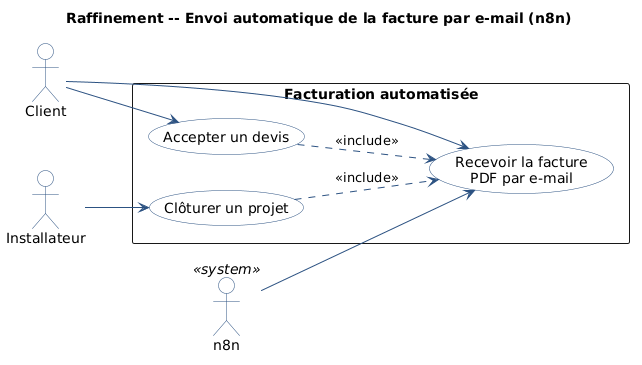
\includegraphics[width=0.92\textwidth]{uc-n8n-facture.png}%
  }{%
    \fbox{\parbox[c][7cm][c]{0.92\textwidth}{\centering
      Compiler \texttt{uc-n8n-facture.puml} $\rightarrow$ \texttt{uc-n8n-facture.png}%
    }}%
  }
  \caption{Diagramme de cas d'utilisation --- envoi automatique facture via n8n}
  \label{fig:uc-n8n-facture}
\end{figure}

\paragraph{Diagramme de séquence.}
La figure~\ref{fig:seq-n8n-facture} détaille les interactions entre le
\texttt{project-service}, n8n, l'endpoint interne PDF et le serveur SMTP
lors de l'acceptation d'un devis (déclencheur principal du sprint~5).

\begin{figure}[H]
  \centering
  \IfFileExists{seq-n8n-facture.png}{%
    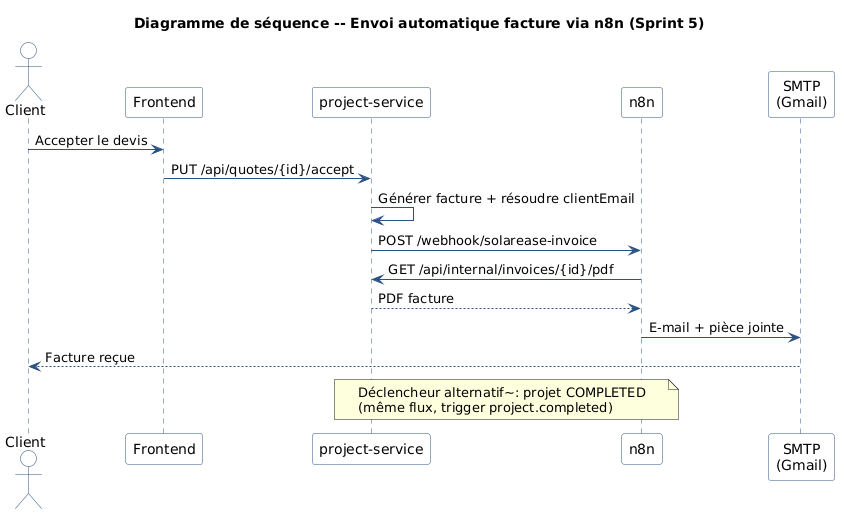
\includegraphics[width=0.95\textwidth]{seq-n8n-facture.png}%
  }{%
    \fbox{\parbox[c][8cm][c]{0.95\textwidth}{\centering
      Compiler \texttt{seq-n8n-facture.puml} $\rightarrow$ \texttt{seq-n8n-facture.png}%
    }}%
  }
  \caption{Diagramme de séquence --- workflow n8n d'envoi de facture PDF}
  \label{fig:seq-n8n-facture}
\end{figure}

\paragraph{Chaîne technique.}
Le flux comporte quatre étapes principales~:
(1)~après \texttt{generateInvoiceFromQuote()} ou passage en
\texttt{COMPLETED}, le \texttt{project-service} envoie un POST JSON au webhook
\texttt{/webhook/solarease-invoice}~;
(2)~n8n vérifie que \texttt{clientEmail} est renseigné~;
(3)~n8n récupère le PDF via
\texttt{GET /api/internal/invoices/\{id\}/pdf} (endpoint interne protégé par
\texttt{X-Internal-Secret}, sans JWT, accessible uniquement sur le réseau
Docker)~;
(4)~n8n envoie l'e-mail via SMTP (Gmail, port~587, STARTTLS) avec la facture
en pièce jointe.

\paragraph{Implémentation.}
Les composants principaux sont~:
\begin{itemize}[leftmargin=*, nosep]
  \item \texttt{N8nInvoiceWebhookService.java}~: construction du payload et
        appel HTTP vers n8n~;
  \item \texttt{InternalInvoiceController.java}~: téléchargement sécurisé du
        PDF pour n8n~;
  \item \texttt{backend/n8n/workflows/send-invoice-email.json}~: workflow
        versionné (webhook, condition e-mail, HTTP Request, envoi SMTP).
\end{itemize}

Le couplage reste faible~: le contrat JSON entre backend et n8n permet
d'ajouter ultérieurement d'autres automatisations (relance impayée,
notification Slack) sans modifier le cœur métier Java.

% ──────────────────────────────────────────────
\paragraph{Raffinement de cas d'utilisation «~Tableau de bord client~»}

\begin{figure}[H]
  \centering
  \IfFileExists{uc-client-dashboard.png}{%
    \includegraphics[width=0.85\textwidth]{uc-client-dashboard.png}%
  }{%
    \fbox{\parbox[c][6cm][c]{0.85\textwidth}{\centering Diagramme de cas d'utilisation -- Tableau de bord client}}%
  }
  \caption{Diagramme de cas d'utilisation pour «~Tableau de bord client~»}
  \label{fig:uc-dashboard-client}
\end{figure}

\subparagraph{Description textuelle du cas d'utilisation «~Consulter le tableau de bord client~»}

\begin{table}[H]
  \caption{Description textuelle du cas d'utilisation «~Consulter le tableau de bord client~»}
  \label{tab:cu-dashboard-client}
  \centering
  \begin{tabularx}{\textwidth}{|L{3.8cm}|X|}
    \hline
    \rowcolor{figblue!10}
    \textbf{Cas d'utilisation} & Consulter le tableau de bord client. \\
    \hline
    \textbf{Acteur initiateur} & Client authentifié \\
    \hline
    \textbf{But du cas} & Permettre au client de disposer d'une vue synthétique unique sur son projet~: progression, devis, factures, documents, messages et notifications. \\
    \hline
    \textbf{Précondition} & Le client est authentifié et possède au moins un projet associé. \\
    \hline
    \textbf{Description du scénario} &
    \textbf{Scénario principal :}\newline
    1. Le client se connecte à son espace.\newline
    2. Le frontend envoie \texttt{GET /api/clients/me/dashboard}.\newline
    3. Le service agrège en parallèle~: projets actifs, devis, factures, notifications non lues.\newline
    4. Le système construit un \texttt{DashboardClientResponse}.\newline
    5. L'écran affiche des cartes KPI, le stepper du projet actif, les liens rapides et les notifications récentes.\\
    \hline
    \textbf{Scénarios alternatifs} &
    \textit{Scénario alternatif 1 -- Aucun projet :}\newline
    \hspace*{6pt}3.1.~Un message d'accueil et un lien vers «~Mes demandes~» sont affichés.\\
    \hline
  \end{tabularx}
\end{table}

\subparagraph{Description textuelle du cas d'utilisation «~Suivre l'avancement du projet~»}

\begin{table}[H]
  \caption{Description textuelle du cas d'utilisation «~Suivre l'avancement du projet~»}
  \label{tab:cu-suivre-projet}
  \centering
  \begin{tabularx}{\textwidth}{|L{3.8cm}|X|}
    \hline
    \rowcolor{figblue!10}
    \textbf{Cas d'utilisation} & Suivre l'avancement de son projet. \\
    \hline
    \textbf{Acteur initiateur} & Client authentifié \\
    \hline
    \textbf{But du cas} & Permettre au client de visualiser la progression de son installation grâce à un \textit{stepper} 5 étapes et au pourcentage d'avancement temps réel remonté par l'installateur. \\
    \hline
    \textbf{Précondition} & Le client est authentifié et son projet est en cours. \\
    \hline
    \textbf{Description du scénario} &
    \textbf{Scénario principal :}\newline
    1. Le client clique sur sa carte projet depuis le dashboard.\newline
    2. Le frontend envoie \texttt{GET /api/projects/\{id\}}.\newline
    3. L'écran affiche un stepper en 5 étapes~: Étude $\rightarrow$ Validation $\rightarrow$ Installation $\rightarrow$ Mise en service $\rightarrow$ Terminé.\newline
    4. Le pourcentage d'avancement (\texttt{currentProgress}) est affiché avec une barre.\newline
    5. Les avancements terrain de l'installateur s'affichent dans une chronologie.\\
    \hline
    \textbf{Scénarios alternatifs} &
    \textit{Scénario alternatif 1 -- Projet annulé :}\newline
    \hspace*{6pt}3.1.~Un bandeau signale le statut \texttt{CANCELLED}.\\
    \hline
  \end{tabularx}
\end{table}

\subsection{Conception du sprint 5}

L'analyse conceptuelle de ce cinquième sprint comprendra la description des
diagrammes de séquence liés aux fonctionnalités majeures du sprint~5. Elle
se conclura par l'élaboration du diagramme de classes, synthétisant
l'ensemble des éléments étudiés.

\subsubsection{Diagrammes de séquence}

Dans cette phase, nous présentons les diagrammes de séquence correspondant
aux principales fonctionnalités développées lors du sprint~5. Ces diagrammes
illustrent les interactions entre les différents composants du système pour
chaque fonctionnalité ciblée.

% ──────────────────────────────────────────────
\paragraph{Diagramme de séquence «~Soumettre une demande solaire~»}

La figure ci-après présente le flux complet d'une demande solaire~:
soumission via le formulaire public, persistance, notification aux admins
et traitement (conversion en projet, demande de compléments ou rejet).

\begin{figure}[H]
  \centering
  \IfFileExists{seq-demande-solaire.png}{%
    \includegraphics[width=0.95\textwidth,height=0.75\textheight,keepaspectratio]{seq-demande-solaire.png}%
  }{%
    \fbox{\parbox[c][7cm][c]{0.92\textwidth}{\centering Diagramme de séquence «~Soumettre une demande solaire~»}}%
  }
  \caption{Diagramme de séquence «~Soumettre une demande solaire~»}
  \label{fig:seq-s5-demande}
\end{figure}

% ──────────────────────────────────────────────
\paragraph{Diagramme de séquence «~Cycle complet du devis~»}

La figure ci-après illustre le cycle de vie du devis~: création (\texttt{DRAFT}),
envoi au client (\texttt{SENT}), acceptation (\texttt{ACCEPTED}) et émission
automatique de la facture (\texttt{INVOICED}).

\begin{figure}[H]
  \centering
  \IfFileExists{seq-cycle-devis.png}{%
    \includegraphics[width=0.95\textwidth,height=0.75\textheight,keepaspectratio]{seq-cycle-devis.png}%
  }{%
    \fbox{\parbox[c][7cm][c]{0.92\textwidth}{\centering Diagramme de séquence «~Cycle complet du devis~»}}%
  }
  \caption{Diagramme de séquence «~Cycle complet du devis~»}
  \label{fig:seq-s5-quote}
\end{figure}

% ──────────────────────────────────────────────
\paragraph{Diagramme de séquence «~Consulter le tableau de bord client~»}

La figure ci-après détaille l'agrégation parallèle des données du dashboard
client~: projets actifs, devis, factures et notifications.

\begin{figure}[H]
  \centering
  \IfFileExists{seq-dashboard-client.png}{%
    \includegraphics[width=0.95\textwidth,height=0.7\textheight,keepaspectratio]{seq-dashboard-client.png}%
  }{%
    \fbox{\parbox[c][7cm][c]{0.92\textwidth}{\centering Diagramme de séquence «~Consulter le tableau de bord client~»}}%
  }
  \caption{Diagramme de séquence «~Consulter le tableau de bord client~»}
  \label{fig:seq-s5-dashboard}
\end{figure}

\subsubsection{Diagramme de classes du sprint 5}

Ce diagramme de classes global illustre l'architecture du projet, avec les
classes liées au sprint~5.

Il permet d'identifier clairement les entités utilisées lors de ce cinquième
sprint.

\begin{figure}[H]
  \centering
  \IfFileExists{class-sprint5.png}{%
    \includegraphics[width=0.85\textwidth]{class-sprint5.png}%
  }{%
    \fbox{\parbox[c][8cm][c]{0.92\textwidth}{\centering Diagramme de classes global du sprint 5}}%
  }
  \caption{Diagramme de classes global du sprint~5}
  \label{fig:class-s5}
\end{figure}

\subsection{Réalisation du sprint 5}

\subsubsection{Extraits de code significatifs}

\begin{lstlisting}[caption={QuoteService.java --- Acceptation et facturation automatique},
                   label=lst:quote-accept, language=Java]
@Service @Transactional @RequiredArgsConstructor
public class QuoteService {

    public QuoteDTO acceptQuote(Long quoteId) {
        QuoteEntity q = quoteRepository.findById(quoteId)
            .orElseThrow(() -> new ResourceNotFoundException("Quote not found"));
        if (q.getValidUntil() != null
            && q.getValidUntil().isBefore(LocalDate.now())) {
            throw new IllegalStateException("Quote has expired");
        }
        q.setStatus(QuoteEntity.QuoteStatus.ACCEPTED);
        q.setAcceptedAt(LocalDateTime.now());
        quoteRepository.save(q);

        // Auto-generate invoice
        InvoiceEntity invoice = generateInvoiceFromQuote(q);
        q.setStatus(QuoteEntity.QuoteStatus.INVOICED);
        quoteRepository.save(q);

        // Notify installer and client
        notificationService.notifyQuoteAccepted(q);
        notificationService.notifyInvoiceGenerated(invoice);
        return mapToDTO(q);
    }

    private InvoiceEntity generateInvoiceFromQuote(QuoteEntity q) {
        InvoiceEntity inv = InvoiceEntity.builder()
            .number("INV-" + java.time.Year.now() + "-"
                + String.format("%05d", new Random().nextInt(99999)))
            .project(q.getProject()).clientId(q.getClientId())
            .installerId(q.getInstallerId())
            .amount(q.getTotalAmount()).status("SENT")
            .date(LocalDate.now())
            .dueDate(LocalDate.now().plusDays(30))
            .quoteId(q.getId()).build();
        return invoiceRepository.save(inv);
    }
}
\end{lstlisting}

\begin{lstlisting}[caption={AccessControlService.java --- Contrôle d'accès multi-rôle},
                   label=lst:access-ctrl, language=Java]
@Service
public class AccessControlService {

    public void requireAnyRole(String userRole, String... allowedRoles) {
        boolean allowed = Arrays.stream(allowedRoles)
            .anyMatch(r -> r.equalsIgnoreCase(userRole));
        if (!allowed) {
            throw new AuthorizationException(
                "Role " + userRole + " is not authorized");
        }
    }

    public void requireClientOwnsResource(String userRole,
            String userId, String resourceClientId) {
        if ("CLIENT".equalsIgnoreCase(userRole)
            && !userId.equals(resourceClientId)) {
            throw new AuthorizationException("Access denied");
        }
    }
}
\end{lstlisting}

\subsubsection{Interfaces utilisateur réalisées}

\begin{figure}[H]
  \centering
  \fbox{\parbox{0.85\textwidth}{
    \centering\vspace{0.5cm}
    \textit{Tableau de bord de l'espace client}\\[4pt]
    \small Remplacer par : \texttt{\textbackslash includegraphics[width=0.85\textbackslash textwidth]\{images/client-dashboard.png\}}\\[4pt]
    KPI (projets actifs, terminés, notifs), projet actif avec barre de progression, liens rapides
    \vspace{0.5cm}
  }}
  \caption{Tableau de bord client -- Sprint 5}
  \label{fig:ui-client-dashboard}
\end{figure}

\begin{figure}[H]
  \centering
  \fbox{\parbox{0.85\textwidth}{
    \centering\vspace{0.5cm}
    \textit{Détail du projet côté client avec stepper et avancement}\\[4pt]
    \small Remplacer par : \texttt{\textbackslash includegraphics[width=0.85\textbackslash textwidth]\{images/client-project-detail.png\}}\\[4pt]
    Stepper 5 étapes (Étude, Validation, Installation, Mise en service, Terminé), barre avancement terrain, devis
    \vspace{0.5cm}
  }}
  \caption{Détail projet espace client avec stepper -- Sprint 5}
  \label{fig:ui-client-detail}
\end{figure}

\begin{figure}[H]
  \centering
  \fbox{\parbox{0.85\textwidth}{
    \centering\vspace{0.5cm}
    \textit{Interface de gestion des devis}\\[4pt]
    \small Remplacer par : \texttt{\textbackslash includegraphics[width=0.85\textbackslash textwidth]\{images/quotes-list.png\}}\\[4pt]
    Liste des devis avec statut (DRAFT, SENT, ACCEPTED, INVOICED), actions contextuelles
    \vspace{0.5cm}
  }}
  \caption{Gestion des devis -- Sprint 5}
  \label{fig:ui-quotes}
\end{figure}

\begin{figure}[H]
  \centering
  \fbox{\parbox{0.85\textwidth}{
    \centering\vspace{0.5cm}
    \textit{Acceptation de devis côté client}\\[4pt]
    \small Remplacer par : \texttt{\textbackslash includegraphics[width=0.85\textbackslash textwidth]\{images/quote-accept.png\}}\\[4pt]
    Carte devis avec détails (main-d'œuvre, matériaux, TVA, total), boutons Accepter / Refuser
    \vspace{0.5cm}
  }}
  \caption{Acceptation de devis par le client -- Sprint 5}
  \label{fig:ui-quote-accept}
\end{figure}

\begin{figure}[H]
  \centering
  \fbox{\parbox{0.85\textwidth}{
    \centering\vspace{0.5cm}
    \textit{Gestion des demandes solaires (côté admin)}\\[4pt]
    \small Remplacer par : \texttt{\textbackslash includegraphics[width=0.85\textbackslash textwidth]\{images/demands-admin.png\}}\\[4pt]
    Liste des demandes avec filtres par statut, actions : compléter, valider, convertir en projet
    \vspace{0.5cm}
  }}
  \caption{Gestion des demandes solaires -- Sprint 5}
  \label{fig:ui-demands}
\end{figure}

\begin{figure}[H]
  \centering
  \fbox{\parbox{0.85\textwidth}{
    \centering\vspace{0.5cm}
    \textit{Liste des factures avec téléchargement PDF}\\[4pt]
    \small Remplacer par : \texttt{\textbackslash includegraphics[width=0.85\textbackslash textwidth]\{images/invoices-list.png\}}\\[4pt]
    Factures auto-générées, numéro INV-2026-XXXXX, statut (DRAFT, SENT, PAID), bouton PDF
    \vspace{0.5cm}
  }}
  \caption{Liste des factures -- Sprint 5}
  \label{fig:ui-invoices}
\end{figure}

\subsection{Environnement des sprints 4 et 5}

\begin{table}[H]
  \caption{Technologies et outils utilisés -- Sprints 4 et 5}
  \label{tab:tech-r3}
  \centering
  \begin{tabularx}{\textwidth}{|L{3cm}|L{3cm}|X|}
    \hline
    \rowcolor{figblue!20}
    \textbf{Technologie} & \textbf{Version} & \textbf{Rôle dans les sprints 4 et 5} \\
    \hline
    Spring WebSocket & 3.2 & Communication temps réel STOMP/SockJS \\
    \hline
    SockJS & 1.x & Fallback WebSocket pour navigateurs incompatibles \\
    \hline
    STOMP & 1.2 & Protocole de messagerie sur WebSocket \\
    \hline
    OpenPDF & 1.3.x & Génération des factures PDF \\
    \hline
    JavaMail & -- & Envoi d'emails d'invitation et notification \\
    \hline
    Twilio & -- & Envoi de SMS d'invitation (stub) \\
    \hline
    Flyway & 10.x & Migrations V1--V12 (devis, factures, demandes, conversations, etc.) \\
    \hline
    React & 18.x & Espace client~: dashboard, stepper, cartes devis \\
    \hline
    Framer Motion & 11.x & Animations du stepper et des transitions de page \\
    \hline
    Sonner & 1.x & Toasts de notification côté frontend \\
    \hline
  \end{tabularx}
\end{table}

\subsubsection{Tests et validation}

\begin{table}[H]
  \caption{Résultats des tests fonctionnels -- Sprint 5}
  \label{tab:tests-s5}
  \centering\small
  \begin{tabularx}{\textwidth}{|C{1.2cm}|L{3.5cm}|X|C{1.4cm}|}
    \hline
    \rowcolor{figblue!20}
    \textbf{ID} & \textbf{Cas de test} & \textbf{Résultat attendu} & \textbf{Statut} \\
    \hline
    T-34 & Demande publique & HTTP 201, statut NOUVELLE & \ok~OK \\
    \hline
    T-35 & Conversion demande & Projet créé, demande VALIDEE & \ok~OK \\
    \hline
    T-36 & Créer devis DRAFT & HTTP 201, numéro auto-généré & \ok~OK \\
    \hline
    T-37 & Envoyer devis & DRAFT$\to$SENT, client notifié & \ok~OK \\
    \hline
    T-38 & Accepter devis & SENT$\to$ACCEPTED$\to$INVOICED, facture créée & \ok~OK \\
    \hline
    T-39 & Refuser devis & SENT$\to$REJECTED, raison enregistrée & \ok~OK \\
    \hline
    T-40 & Devis expiré & Acceptation refusée, HTTP 400 & \ok~OK \\
    \hline
    T-41 & Facture PDF & PDF valide généré, téléchargement OK & \ok~OK \\
    \hline
    T-47 & Envoi n8n facture & Webhook OK, e-mail reçu à \texttt{clientEmail} & \ok~OK \\
    \hline
    T-42 & Dashboard client & KPI affichés, projet actif en avant & \ok~OK \\
    \hline
    T-43 & Stepper client & Progression synchronisée avec statut & \ok~OK \\
    \hline
    T-44 & Accès non autorisé & HTTP 403, client ne voit que ses données & \ok~OK \\
    \hline
    T-45 & CRUD installateurs & Création, modification, suppression admin & \ok~OK \\
    \hline
    T-46 & Invitation client & Email envoyé avec lien d'inscription & \ok~OK \\
    \hline
  \end{tabularx}
\end{table}

\begin{conclusionbox}
Les sprints 3, 4 et 5 finalisent la plateforme SolarEase en la dotant de toutes les
fonctionnalités nécessaires à une exploitation opérationnelle. Le suivi
terrain temps réel permet à l'installateur de communiquer son avancement
depuis le chantier. La messagerie et les notifications assurent une
collaboration fluide entre les trois rôles (admin, installateur, client).
L'espace client offre une expérience dédiée avec un suivi visuel du projet
à travers un stepper intuitif. Enfin, le workflow commercial complet ---
de la demande solaire à la facturation automatique en passant par le devis,
puis l'envoi de la facture PDF par e-mail via n8n (section~\ref{sec:n8n}) ---
transforme SolarEase en une solution professionnelle de gestion de projets
solaires, prête pour le marché tunisien.
\end{conclusionbox}

\cleardoublepage
